\documentclass[10pt,aps,pra,reprint,amsmath,amsfonts,amssymb,showpacs]{revtex4-1}
\usepackage{epsfig,psfrag,graphicx,bm,color}

%\def\del#1{{}}
\def\del#1{{\bf (DELETED TEXT)}}
%\def\C#1{#1}
\def\C#1{{\bf #1}}


% --- journals --- %
\newcommand{\aap}{A{\&}A}
\newcommand{\aaps}{A{\&}AS}
\newcommand{\aj}{AJ}
%\newcommand{\apj}{ApJ}
\newcommand{\apjl}{ApJL}
\newcommand{\apjs}{ApJS}
\newcommand{\apss}{Ap{\&}SS}
\newcommand{\araa}{ARA{\&}A}
%\newcommand{\prd}{Phys. Rev. D}
%\newcommand{\pre}{PRE}
\newcommand{\mnras}{MNRAS}
\newcommand{\ssr}{SSRv}
%\newcommand{\nat}{Nature}
\newcommand{\physrep}{Phys.~Rep.}
\newcommand{\jcomp}{J.~Comput.~Phys.}
\newcommand{\jcap}{JCAP}

%NEW
\newcommand{\bx}{{\bf x}}
\newcommand{\fg}{{F_\gamma}}
\newcommand{\sg}{{S_\gamma}}
\newcommand{\psf}{\theta_\rmn{res}}
\newcommand{\ph}{{\rm ph}}
\newcommand{\eph}{E_\ph}
\newcommand{\nph}{N_\ph}
\newcommand{\vir}{{\rmn vir}}
\newcommand{\gal}{{\rmn gal}}
\newcommand{\iruv}{{\rmn sd}}
\newcommand{\clu}{{\rmn cl}}
\newcommand{\sfe}{{\rmn sfe}}
\newcommand{\sub}{{\rmn sub}}
\newcommand{\msun}{{M_\odot}}

%OLD
\newcommand{\beq}{\begin{equation}}
\newcommand{\eeq}{\end{equation}}
\newcommand{\rmn}{\mathrm}
\newcommand{\GeV}{\,{\rm GeV}}
\newcommand{\TeV}{\,{\rm TeV}}
\newcommand{\eV}{\,{\rm eV}}
\newcommand{\dd}{\mathrm{d}}
\newcommand{\mx}{\ensuremath{m_{\chi}}}
\newcommand{\ga}{\gamma}
\newcommand{\ngamma}{\ensuremath{N_{\gamma}}}
\newcommand{\ngammai}{\ensuremath{N_{\gamma,i}}}
\newcommand{\sigmaannv}{\ensuremath{\langle\sigma v\rangle}}
\newcommand{\sigv}{\ensuremath{\sigma_v}}
\newcommand{\ic}{\mathrm{IC}}
\newcommand{\egamma}{\ensuremath{E_{\gamma}}}
\newcommand{\dic}{\mathrm{dIC}}
\newcommand{\fsr}{\mathrm{FSR}}
\newcommand{\CR}{\mathrm{CR}}
\newcommand{\rhos}{\ensuremath{\rho_s}}
\newcommand{\rs}{\ensuremath{r_s}}
\newcommand{\rvir}{r_{200}}
\newcommand{\mvir}{M_{200}}
\newcommand{\rhoc}{\ensuremath{\rho_c}}
\newcommand{\B}{\rmn{B}}
\newcommand{\e}{\rmn{e}}
\newcommand{\eg}{E_\gamma}
\newcommand{\ir}{\rmn{ir}}
\newcommand{\Km}{\rmn{K}`}
\newcommand{\Imm}{\rmn{I}`}
\newcommand{\Jm}{\rmn{J}^*}
\newcommand{\Jmm}{\rmn{J}`}

\begin{document}

\title{Prospects of detecting gamma-ray emission from galaxy clusters:
  cosmic rays and dark matter annihilations}

\author{Anders Pinzke$^{1}$} \email{apinzke@physics.ucsb.edu} 
\author{Christoph Pfrommer$^{2}$}\email{pfrommer@cita.utoronto.ca}
\author{Lars Bergstr\"om$^{3}$}\email{lbe@fysik.su.se}


\affiliation{$^{1}$University of California - Santa Barbara,
  Department of Physics, CA 93106-9530, USA}

\affiliation{$^{2}$Heidelberg Institute for Theoretical Studies (HITS), Schloss-Wolfsbrunnenweg 33, DE - 69118 Heidelberg, Germany}

\affiliation{$^{3}$The Oskar Klein Centre for Cosmoparticle Physics, Department
  of Physics, Stockholm University, AlbaNova University Center, SE - 106 91
  Stockholm, Sweden}

\date{\today}

\pacs{95.35.+d, 95.85.Pw, 98.62.Gq, 98.65.-r, 98.70.Sa}


\begin{abstract}
... to be written...
\end{abstract}

\maketitle
\section{Introduction}

Dark matter has been searched for in direct detection experiments
\cite{Pato:2010zk}, at accelerators
\cite{Ellis:2001hv,Baer:2006ff,Khachatryan:2011tk} and also in
indirect detection experiments looking for signals in the cosmic-ray
spectra of antiprotons, positrons, neutrinos and all of the
electromagnetic spectrum from radio waves to gamma rays
\cite{Bergstrom:2009ib}. So far, the improvements in direct detection
sensitivity have put this method into focus, but the situation may
change considerably the coming few years as the CERN LHC experiments
collect data, and new gamma-ray detectors are being planned, such as
the CTA \cite{Consortium:2010bc}. In fact, it has recently been
pointed out \cite{Bergstrom:2010gh} that a dedicated ground-based
gamma-ray detector would have potential that goes far beyond that of
the other methods, depending on presently unknown parameters in the
particle physics models for dark matter.


Among the astrophysical systems which will be very interesting to
detect, and study, with coming gamma-ray detectors (Fermi, HESS,
MAGIC, VERITAS, and eventually large detectors like CTA) belong galaxy
clusters. The most promising directions in which to search for a
gamma-ray annihilation signal (from the annihilation process itself,
and also the accompanying bremsstrahlung and inverse Compton
components coming from charged particles produce in the annihilations)
are basically three:

1. The galactic centre (g.c.). This is where all numerical simulations
of cold dark matter predict the highest density. However, the detailed
dark matter density in the very central part is difficult to predict,
due a to a possibly very complicated interplay between baryons, dark
matter, and the central galactic black hole. Also, it is a very
crowded region with many gamma-ray sources like pulsars and other
supernova recants, which have to be subtracted from the data to
extract the dark matter induced signal. In fact, there is a recent
claim of an indication of a relatively light dark matter particle
contribution to the gamma-ray flux from the
g.c. \cite{2010arXiv1010.2752H}, but other hypotheses seem to work at
least as well \cite{2010arXiv1012.5839B}.

2. The dwarf spheroidal galaxies orbiting the Milky Way, like Segue-1,
Ursa Minor, Draco, Sagittarius, Sculptor, Carina or Willman-1
\cite{2009JCAP...01..016B,2010ApJ...720.1174A,2010JCAP...01..031S,2010JCAP...01..031S}. The
problem here is that the nature of many of these small, dark
matter-dominated galaxies is not entirely clear, and the velocity
dispersion estimates are based on rather small numbers of stars. Tidal
disruption and confusion with star clusters are other
complications. Thus the dark matter density profile is very uncertain
for most of them. Nonetheless, by stacking the data together from many
dwarf spheroidals these uncertainties can be made less severe, and
preliminary results from Fermi-LAT shows this method to give quite
promising results \cite{garde}.

3. Galaxy clusters. This possibility has been less studied, however we
noted in a previous Letter \cite{2009PhRvL.103r1302P} that the are
certain advantages that work in favour of this possible target for
gamma-ray detection of dark matter annihilation.  Galaxy clusters
constitute the most massive objects in our Universe that are forming
today. This causes their DM subhalo mass function to be less affected
by tidal stripping compared to galaxy sized halos that formed long
ago.  The annihilation luminosities of the DM halo component for
e.g. the Virgo cluster and the Draco dwarf scales in a way (see
\cite{2009PhRvL.103r1302P}) that the ratio of gamma-ray luminosities
from the smooth components is around 4, in favour of Virgo. In
addition, there may be a further enhancement due to substructure,
which to a large extent should be unaffected by tidal disruption, at
least in the outer regions.  According to a recent estimate
\cite{2011MNRAS.410.2309G}, more massive haloes tend to have a larger
mass fraction in subhalos.  For example, cluster size haloes typically
have 7.5 per cent of the mass within $r_{200}$ in substructures of
fractional mass larger than $10^{-5}$, which is 25 per cent higher
than galactic haloes \footnote{All halo masses and length scales in
  this paper are scaled to the currently favored value of Hubble's
  constant, $H_0 = 70\, \rm{km~s}^{-1}\,\rm{Mpc}^{-1}$. We define the
  virial mass $\mvir$ and virial radius $\rvir$ as the mass and radius
  of a sphere enclosing a mean density that is 200 times the critical
  density of the Universe $\rho_{\rm{cr}}$.}.

For a satellite dwarf galaxy, however, once it is accreted by the
Milky Way, the outer regions are severely affected by tidal
stripping. The longer a satellite has been part of our Galaxy, and the
closer it comes to the center during its pericentral passage, the more
material is removed \cite{2004MNRAS.355..819G}.

In this paper, we will investigate in some more detail the potential
of several of the most promising galaxy clusters to yield an
annihilation gamma-ray yield which could be observable with present
and planned gamma-ray detectors.

For previous work related to dark matter in clusters, see, e.g.,
\cite{2006A&A...455...21C,2009PhRvD..80b3005J}. 


%***********************************************
{\bf Anders, insert your flux table for various clusters, and discuss it}

This yields Fornax ($\mvir=10^{14}\,\msun$) and Virgo
($\mvir=2.1\times10^{14}\,\msun$) \cite{} as the prime targets for DM
observations, Perseus ($\mvir=7.7\times10^{14}\,\msun$) for CR induced
emission and we additionally decide in favor of the well studied
cluster Coma ($\mvir=1.4\times10^{15}\,\msun$) for comparison.


% --- section:  --- %
\section{Theory}
\label{sect:theory}

\subsection{Astrophysics}
\label{sect:AP}

The differential photon flux within a given solid angle $\Delta
\Omega$ along a line-of-sight (los) is given by
\begin{equation}
\label{eq:dflux}
\frac{\dd \fg}{\dd \eg} \equiv \frac{\dd^3 \ngamma}{\dd A \,\dd t\, \dd
  \egamma} = \frac{1}{2}\int_{\Delta\Omega} \dd\psi \sin\psi \frac{\dd \sg}{\dd \eg}(\psi,\eg)\,,
\end{equation}
where
\begin{equation}
\label{eq:dtildeflux}
\frac{\dd \sg}{\dd \eg}(\psi,\eg) = \int_{\Delta\Omega} \dd\Omega \int_{\rm los}
\dd l\, q_{\rm sum}\left(\eg,r\right)\Lambda(\theta)\,,
\end{equation}
and $\sg(\psi, >\eg)$ denotes the surface brightness above the photon
energy $\eg$.  The integration along the line-of-sight $l$, in the
direction $\psi$ that the detector is pointing, is parameterized such
that the radius of the source $r=\sqrt{l^2+D^2-2Dl\cos\Psi}$, where
$D$ is the distance to the source from the galactic center and
$\cos\Psi\equiv\cos\theta\cos\psi-\cos\varphi\sin\theta\sin\psi$. The
angular integration $\dd \Omega= \sin\theta\dd \theta \,\dd \varphi$
is performed over a cone centered around $\psi$ and the opening angle
$\Delta \Omega$ is typically taken to be a few times the point spread
function (PSF) $\psf$. The limited angular resolution results in a
probability that a photon coming from a direction $\psi$' is instead
reconstructed to a direction $\psi$, where the underlying probability
distribution follow a Gaussian:
\begin{equation}
\Lambda(\theta)=\frac{1}{2\pi\psf^2}
\,\rmn{exp}\left[-\frac{\theta^2}{2\psf^2}\right]\,,
\quad \rmn{where}\quad \theta=\psi'-\psi \,.
\end{equation}
We denote the dark matter source function from the smooth halo by
$q_{\rm sum}\left(\eg,r\right)$ where we include contributions from
three main processes; leptophilic DM annihilating to $\mu^+/\mu^-$
decaying to $\rm{e}^+/\rm{e}^-$ pairs that up-scatter background
photons (IC), leptophilic DM emitting final state radiation (FSR), DM
benchmark models where neutralino annihilations generate electrons
that up-scatter background photons (BM-IC) and emit a continuum as
well as final state radiation (BM-Cont). The DM source function is
given by:
\begin{equation}
q_\rmn{sum} \left(\eg,r\right) =
\sum_i q_i\left(\eg,r\right)\B_{\rmn{F},i}\left(\sigv\,,r\right)
\end{equation}
where the source function for each process is written on the form:
\begin{equation}
\quad q_i \left(\egamma,r\right) =
\frac{\dd \ngammai}{\dd E_\gamma} \Gamma_i(r)\,.
\end{equation}
We represent the annihilation rate density with $\Gamma_i =
(\rho/\mx)^2 \, \sigmaannv_i/2$, where $i$ runs over all $\gamma$-ray
producing channels each with the spectrum $\frac{\dd
  \ngammai}{\dd\eg}$ and annihilation cross-section $\sigmaannv_i$.
The DM density is modeled by an Einasto density profile
\begin{equation}
\rho_{\rm Einasto}(r) = \rho_{-2}\cdot \exp\left[- \frac{2}{\alpha}
  \left( \left(\frac{r}{r_{-2}}\right)^\alpha -1 \right) \right],\,
\alpha=0.17 \,,
\end{equation}
that is slightly shallower than the conventional Navaro-Frenk-White
(NFW) profile in the center, but provide a better fit to simulated DM
halos \cite{2010MNRAS.402...21N}. We denote the density where the
density profile has a slope of $-2$ by $\rho_{-2}$, and the radius by
$r_{-2}$. Assuming that all the flux from an NFW profile originate
from within the scale radius $\rs=\rvir/c$, and all the flux from an
Einasto profile originate within $r_{-2}=\rvir/c$, it follows that
$\rho_{-2} = \rhos/4$. The virial radius $\rvir$ of a halo is defined
to be the radius at which the mean density within is a factor
$\Delta=200$ times the critical density $\rhoc$ of the universe. The
characteristic density of the NFW profile $\rhos=(\Delta\rhoc/3)\,
c^3/(\log(1+c)-(c/(1+c)))$, where the mass dependence of the
concentration parameter $c$ is derived from a power-law fit to
cosmological simulations with $\mvir \gtrsim 10^{10} \msun$
\cite{2008MNRAS.391.1940M},
\begin{equation}
\label{eq:cfit}
  c=3.56 \times \left(\frac{\mvir}{10^{15}\,\msun}\right)^{-0.098}\,.
\end{equation}
Note that Eqn.~\ref{eq:cfit} agrees well with
\cite{2009ApJ...707..354Z} for cluster-mass halos after converting the
concentration definitions according to \cite{2003ApJ...584..702H}.

\subsubsection{Substructures}
\label{sect:subst}
\del{The product of enhancement factors from SFE $\B_\sfe(\sigv)$ and
  from substructure enhancement over the smooth halo contribution
  $\B_\sub\left(r\right) = 1+q_\sub(r)/q_\rmn{i}(r)$ is denoted by
  $\B_{\rmn{F}_{,i}}(r,\sigv) = \B_\sfe (\sigv)\,\B_\sub(r)$.}
High-resolution DM simulations of the Milky Way (MW) find vast amount
of substrucures in the outer part of DM halos. Since the annihilating
DM depends on the density squared, the resulting flux is boosted
compared to the smooth density distribution. Recent simulations
suggest a boost from substructures of the order of ten up to a few 100
\cite{2008MNRAS.391.1685S, 2008JPhCS.125a2008K} for a MW size
halo. Based on the result from \cite{2008Natur.456...73S}, we find the
best fit to the luminosity from smooth substructures
(i.e. substructures within substructures are not included) inside
radius $r$ with
\begin{equation}
  {\rm L_{sub}}(<r)= 0.76\,C_1\,C_2(\mvir)\,{\rm L_{200sm}}\,x^{0.95
    \displaystyle{x}^{-0.27}}\,,
  \label{eq:LSub}
\end{equation}
where ${\rm L_{200sm}}$ is the luminosity from the smooth halo without
substructures within $\rvir$ and $x=
\left(\frac{r}{\rvir}\right)$. The first normalization constant is
given by
\begin{equation}
  C_1=\left(\frac{M_{\rm res,sim}}{M_{\rm lim}}\right)^{0.226}\,,
   \label{eq:C1}
\end{equation}
where $M_{\rm res,sim}=10^5\msun$ is the minimum subhalo mass in the
MW simulation, and $M_{\rm lim}$ the free streaming mass. Here we
assume that the power-law scaling relation in Eqn.~\ref{eq:C1} is
valid down to the minimum mass of DM halos, which is conventionaly in
the cold dark matter universe
\cite{2001PhRvD..64h3507H,2005JCAP...08..003G} taken to be
$10^{-6}\msun$ . Note that potentially the power-law could flatten
torwards smaller mass scales although current simulations show no hits
of such a behaviour and in addition we are approaching the asymptotic
behavior in the power spectrum on these scales(CHECK). For DM halos
more (less) massive than the MW we expect a larger (smaller) boost
from substructures, simply because the larger (smaller) mass range
down to the minimum mass $M_\rmn{lim}$. We capture this halo mass
dependence with the second normalization in Eqn.~\ref{eq:LSub}:
\begin{equation}
C_2(\mvir)=\left(\frac{\mvir}{M_{\rm 200sim}}\right)^{0.226}\,,
 \label{eq:C2}
\end{equation}
where $M_{\rm 200,sim}=1.9\times10^{12}\msun$ is the mass of the MW
halo in the simulation \cite{2008Natur.456...73S}. Note that our
approach of fitting the scaling behavior of
$\rmn{L_{sub}}(M_\rmn{lim})$ directly from numerical simulations
self-consistently accounts for the radial dependence of the
substructure concentration \cite{2008MNRAS.391.1685S}. The boost from
the substructures is finally derived from
\begin{equation}
   \mathrm{B_{sub}}\left(r\right) = 
\frac{1}{\mathrm{L_{sm}}(r)}\frac{\dd \mathrm{L_{sm,sub}}}{\dd\mathrm{V}}\,.
  \label{eq:BoostSub}
\end{equation}
DISCUSS FIGURES

\begin{figure}%[t]
 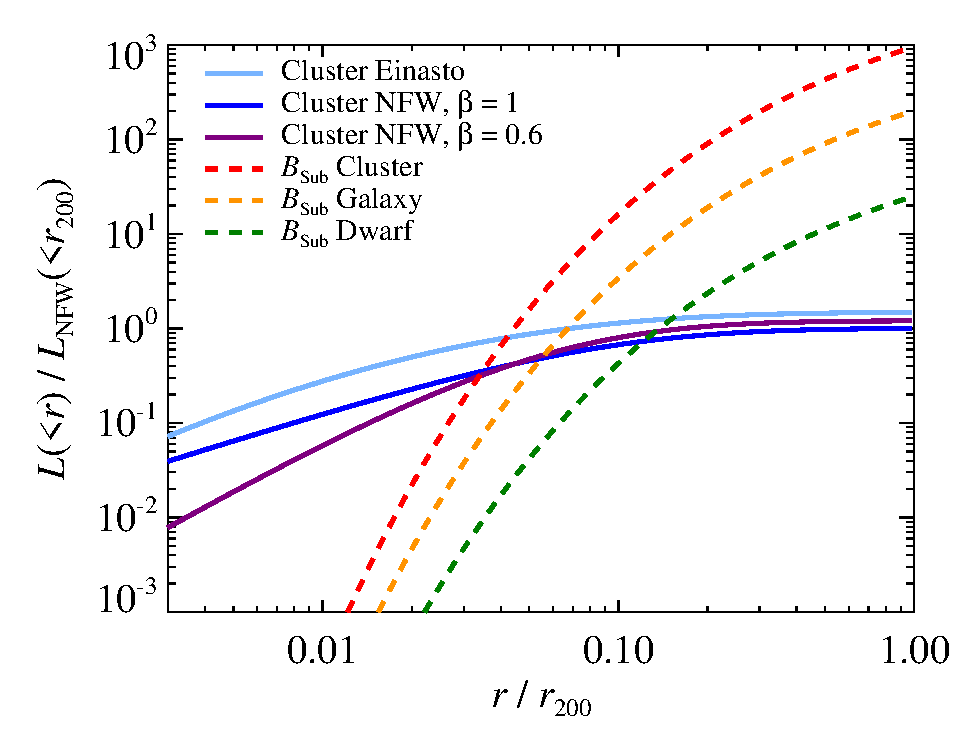
\includegraphics[width=0.99\columnwidth]{figures/dens.prof.eps}
\caption{\it The radial dependence of various luminosity
  contributions. The solid lines show the accumulative smooth
  luminosity from three different density profiles for a cluster with
  the mass $\mvir=10^{15}\,\msun$; Einasto profile with
  $\alpha=0.17$ (light blue), cuspy NFW profile with $\beta=1.0$ (dark
  blue), core NFW profile with $\beta=0.6$ (purple). The dashed lines
  show the accumulative luminosity from substructures for three
  different mass scales; an $\mvir=10^{15}\,\msun$ galaxy cluster
  (red), an $\mvir=10^{12}\,\msun$ galaxy (orange), and an
  $\mvir=10^{8}\,\msun$ dwarf galaxy (green). All luminosities have
  been normalized with the luminosity from a cuspy NFW profile within
  $\rvir$. Note the large expected boost from substructures in
  clusters ($\sim1000$), and the relative small boost in dwarf
  galaxies ($\sim20$).}
 \label{fig1}
\end{figure}

\begin{figure}
  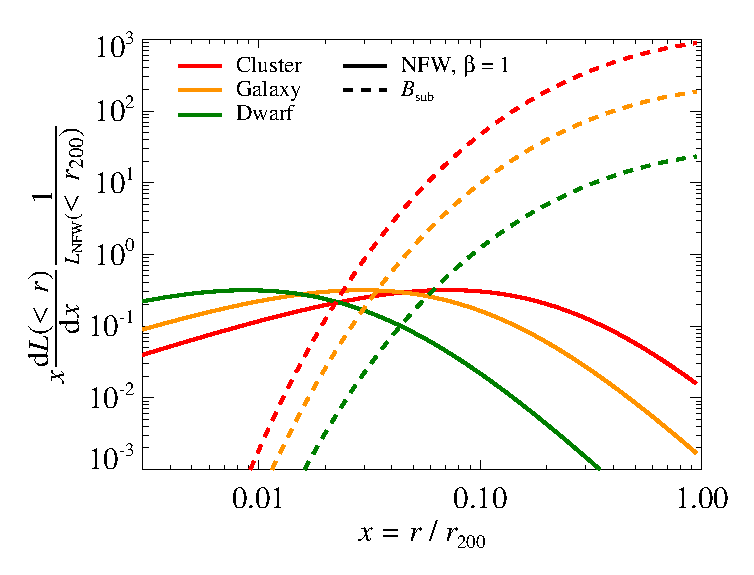
\includegraphics[width=0.99\columnwidth]{figures/emissiv.sub.eps}
  \caption{\it Volume weighted luminosity for different at different
    scales. The solid lines show the emissivity from a NFW density
    profile for three different mass scales; a $\mvir=10^{15}\,\msun$
    galaxy cluster (red), a $\mvir=10^{12}\,\msun$ galaxy (orange), a
    $\mvir=10^{8}\,\msun$ dwarf galaxy (green). The dashed lines show
    the emissivity from substructures for the same three mass
    scales. All emissivities have been normalized with the luminosity
    from a NFW profile within $\rvir$.}
  \label{fig2}
\end{figure}

\subsubsection{Cosmic-ray induced gamma-ray emission}
\label{sect:CRs}
The formation process of a galaxy cluster is a very energetic
processes that induces both turbulence as well as frequently occurring
merging and accretion shocks. These processes are thought to
accelerate large quantities of relativistic non-thermal electrons and
protons to high energies. On smaller scales, such as galaxies, there
is convincing evidence of such non-thermal populations. Especially, in
the MW, the cosmic rays are observed directly as well as indirectly
through radio, X-ray, and gamma-ray emission. On larger scales of the
order of few 100 kpc up to Mpc, there are a vast number of
observations of radio emission coming from radio mini halos in the
center of cooling flow clusters, radio relics in the periphery of
clusters \cite{2004rcfg.proc..335K} as well smooth giant radio halos
that have been observed in more than 50 clusters
\cite{2003ASPC..301..143F,2008SSRv..134...93F}. This emission is
expected to emerge from synchrotron emitting cosmic-ray electrons
although the precise origin of especially the electrons in giant radio
halos is still not settled. If the electrons are of hadronic origin,
which seems quite natural due to the long cooling time of cosmic ray
protons (CRs) that allows for both an extended and large population of
CRs to build up over the cluster history \cite{1997ApJ...487..529B}.

When the CRs interact with ambiant gas protons, it results in the
production of both charged and neutral pions that decay into
electrons, neutrinos, and gamma-rays. The cluster gamma-ray emission
is crucial in this respect as it potentially provides the unique and
unambiguous evidence of CR populations in clusters through observing
the $\pi^0$ bump at about 100~MeV in the spectra. We adopt the
spectrally and spatially universal gamma-ray model developed by Pinzke
\& Pfrommer \cite{2010MNRAS.409..449P} to estimate the emission from
decaying $\pi^0:s$ that dominates over the inverse Compton emission
from primary and secondary electrons above 100~MeV in clusters. The
gamma-ray formalism was derived from high resolution simulations of
clusters of galaxies that included radiative hydrodynamics, star
formation, supernova feedback, and followed CR physics using a novel
formulation that trace the most important injection and loss processes
self-consistently while accounting for the CR pressure in the equation
of motion
\cite{2008A&A...481...33J,2007A&A...473...41E,2006MNRAS.367..113P}.
We note that the overall normalization of the CR and gamma-ray
distribution scales with the maximum acceleration efficiency at
structure formation shock waves. Following recent observations at
supernova remnants \cite{2009Sci...325..719H} as well as theoretical
studies \cite{2005ApJ...620...44K}, we adopt a realistic value of this
parameter and assume that 50\% of the dissipated energy at strong
shocks is injected into CRs while this efficiency rapidly decreases
for weaker shocks \cite{2007A&A...473...41E}.
 
The gamma-ray source function from decaying $\pi^0:s$ induced by CRs
interacting with ambient gas  $q_\CR \propto \rho_\rmn{gas}
rho_\CR$

mention that gamma rays induced by protons are especially
good targets for cherenkov telescopes since the emission trace the gas
density and CR denity



\subsection{Particle physics}

\subsubsection{Leptophilic models}
Sommerfeld enhancement, electron spectra

\subsubsection{Supersymetric dark matter}
neutralino, benchmark models, continuum emission, electron spectra 

\subsubsection{Final state radiation}
The photon spectrum from resulting from FSR is universal with only a
weak dependence of the underlying particle physics model. The photon
yield from this process is given by (see
e.g. \cite{2008JHEP...01..049B})
\begin{equation}
\frac{\dd N_{X \bar{X}}}{\dd x} \approx \frac{\alpha Q_X^2}{\pi}
\mathcal{F}_X(x) \log\left[\frac{4 m_\chi^2\left(1-x\right)}{m_X^2}\right]\,.
\end{equation}
Here, the normalized photon energy $x=\eg/m_\chi c^2$, $\alpha =
e^2/\hbar c$ is the fine-structure constant, $Q_X^2$ and $m_X$ the
charge and mass of the particle $X$, respectively. The function
$\mathcal{F}_X(x)$ depends on the spin of the final state and is given
by
\begin{equation}
\mathcal{F}_\rmn{fermion}(x) = \frac{1+\left(1-x\right)^2}{x}\,
\end{equation}
for fermions. 


\subsection{Radiative processes}

\subsubsection{Inverse Compton}
The source function of inverse Compton emission resulting from DM
annihilating is given by
\begin{equation}
  q_{\rm IC}\left(E_\gamma, r\right) = \int
  \dd E_\e\, \frac{\dd n_\e}{\dd E_\e} 
  P_{\rm IC}\left(E_\gamma,E_\e\right) ,
  \label{eq:ICemiss}
\end{equation}
where $P_{\rm IC}$ is derived by convolving the IC cross-section with
the differential target photon number density:
\begin{eqnarray}
\label{eq:KN_spec}
P_\rmn{IC} &=&
\frac{3\sigma_\rmn{T}m^2_\e c^5}{4E_\e^2}
\int\frac{n_\rmn{ph}(\eph)\dd \eph}{\eph}\nonumber \\
&\times&\left[2q
  \ln{q}+(1+2q)(1-q)+ \frac{1}{2}\frac{\left(\Gamma_\e q\right)^2}
     {1+\Gamma_\e q}\left(1-q\right)\right]\,,\nonumber \\
&&
\end{eqnarray}
where
\begin{equation}
\Gamma_\e=\frac{4\eph E_\e}{\left(m_\e c^2\right)^2}\,,\qquad \rmn{and} \qquad  
q=\frac{\eg}{\Gamma_\e(E_\e-\eg)}\,.
\end{equation}
We account for two major contributions to the radiative background
field $n_\ph$; the IR and UV light coming from emitting dust and
starlight where $n_\ph\equiv\frac{\dd^2 N_\ph^\clu}{\dd V \,\dd
  \eph}(\eph,r)= \frac{u_\iruv^\clu(\eph,r)}{\eph^2}$ and
$u_\iruv^\clu(\eph,r)$ is given by Eqn.~\ref{eq:E_IR_UV}. We model the
CMB photon spectrum as a photon gas that is isotropically distributed and
follows a black body spectrum with temperature $T$:
\begin{equation}
\label{eq:photon_gas}
  n_\rmn{ph}(\eph) = \frac{\dd^2 N_\ph}{\dd V \,\dd \eph} =
  \frac{1}{\pi^2(\hbar c)^3}\frac{\eph^2}{\exp(\eph/k_\B T)-1}\,.
\end{equation}
Here the the typical energy of a photon before scattering is given by
$<E_\ph>=\epsilon_\ph/n_\ph\approx\,2.70 k_\B T$, where $n_\ph$ and
$\epsilon_\ph$ are the number- and energy-density derived by
integrating $n_\ph(E_\ph)$ and $E_\ph n_\ph(\eph)$ over the photon
energy $\eph$, respectively.

The equilibrium spectrum of the electrons plus positrons in
Eqn.~\ref{eq:ICemiss} is given by $\frac{\dd n_\e}{\dd E_\e}$ and
derived from the CRe diffusion equation:
\begin{eqnarray}
\label{eq:CRdiffusion}
\frac{\partial}{\partial t}\left(\frac{\dd n_\e}{\dd E_\e}\right) = 
&\nabla& \left[D\left(E_\e,\bx\right)\nabla\frac{\dd n_\e}{\dd E_\e}\right] + 
\frac{\partial}{\partial E_\e}
\left[b\left(E_\e,\bx\right) \frac{\dd n_\e}{\dd E_\e}\right]
 \nonumber \\
&+& Q(E_\e,\bx)\,,
\end{eqnarray}
where $D(E_\e,\bx)$ the diffusion coefficient and $b(E_\e,\bx)$ the
electron energy loss term. The source function $Q(E_\e,\bx)$ shows
the number of particles produced per unit time, energy and volume
element that are produced at the position $\bx$:
\begin{equation}
Q(E_\e,r)=\sum_f\frac{\dd N_\e^f}{\dd E_\e}(E_\e) B_f \Gamma(r)\,.
\end{equation}
The subscript $f$ ...(see cola), and $B_f$ is the branching factor.
Here $\frac{\dd N_\e^f}{\dd E_\e}$ denote the differential number of
electrons plus positrons resulting from an annihilation event. For
neutralinos annihilating directly into an electron and positron we
model the differential spectrum with $\frac{\dd N_\e^f}{\dd E_\e}=
2\delta(E_\e-m_\chi c^2)$. We use DarkSUSY to compute both the spectra
when neutralinos annihilate directly into a $\mu^+$ and $\mu^-$ in
the leptophilic model as well as in the four BM models where a
fraction of the annihilating neutralinos is converted into electrons
and positrons (see \cite{2009JCAP...01..016B} and references therein,
also see fit).  

The electrons and positrons loose their energy on a timescale that is
shorter than the diffusive timescale in the ICM of galaxy clusters for
CRe energies above MeV (CHECK). Hence, we neglect the first term of
the r.h.s. in Eq.~\ref{eq:CRdiffusion}, and derive an expression for
the equilibrium number density:
\begin{eqnarray}
{\frac{\dd n_\e}{\dd E_\e}}\left(E_\e, r \right) &=&
 \frac{1}{b(E_\e, r)} \int_{E_\e}^{\mx c^2} \dd E_\e' \, 
  Q(E_\e', r),
\label{eq:nds}\\
b(E_\e,r) &=& \tilde{b}
\left[\frac{B^2_{\rm CMB}}{8\pi}+\frac{B^2(r)}{8\pi}+u_\iruv(r)\right] E_\e^2\,,
\\\tilde{b}&=&\frac{4\sigma_{\rm T}c}{3(m_{\rm e}c^2)^2}\,.
\end{eqnarray}
Here we have included three main loss processes for the electrons;
$B_{\rm CMB}=3.24(1+z)^2\mu {\rm G}$ denotes the equivalent field
strength of the CMB, we parameterize the magnetic field of the galaxy
cluster by $B(r) = 3\mu\rmn{G} \,[n_{\rm e}(r)/n_{\rm e}(0)]^{0.7}$,
which follows from flux frozen magnetic fields. In the following
subsection we derive a semi-analytic formula that estimates the
energy density of the dust and starlight component $u_\iruv(r)$
given by Eqn.~\ref{eq:E_IR_UV}.

{\bf IC -- dust and starlight}\\
Galaxy clusters are typically characterized by the hot gas in the ICM
and the collection of gravitationally bound galaxies. The emission in
the IR and UV wavelengths emerge from dust and starlight in both the
galaxies and the ICM (e.g. \cite{2006ApJ...648L..29P} and
\cite{2009MNRAS.399.1694G}). Most of this radiation leaks out from the
galaxy into the ICM, which explains the very similar spectral shape
for these wavelengths. We use the light from galactic dust and
starlight that is emitted in the IR and UV band and is accurately
measured for the ISM \cite{2006ApJ...648L..29P}. We model these
spectra through a fit to the galactic spectra presented in
\cite{2006ApJ...648L..29P}. We extract the spatial cluster profile of
the emission from a stacked analysis of Sloan Digital Sky Survey
(SDSS) data at the redshift $\sim 0.25$
\cite{2005MNRAS.358..949Z}. Finally, we derive the normalization for
the emission from the galaxy cluster using the IR to X-ray luminosity
relation presented in the IR cluster luminosity analysis
\cite{2008A&A...490..547G}.

{\bf Spectra -- galactic} \\
best fit, IR with a power-law function, UV with three power laws,
similar to Porter, vary normalization to account for uncertainties,
taken at $r=0$ in the galaxy
\begin{eqnarray}
  \eph^2\frac{\dd^2 N_\ph^\gal}{\dd \eph \dd V}
  &\equiv& u_\iruv^\gal(\eph) \nonumber \\ 
  &=& u_\rmn{ir}^\gal(\eph) +  u_\rmn{uv}^\gal(\eph)  \nonumber \\ 
  \\
  u_\rmn{uv}^\gal(\eph) &=& \frac{23\,\rmn{eV}}{\rmn{cm}^3} 
  \left(\frac{1.23\,\rmn{eV}}{\eph}\right)^{1.9} \nonumber \\
  &\times&\left[1+\left(\frac{2.04\,\rmn{eV}}{\eph}\right)^{20}\right]
  ^{-\frac{1.9}{20}}\nonumber \\
  &\times& \left[1+\left(\frac{0.78\,\rmn{eV}}{\eph}\right)^{20}\right]^{-\frac{2.6}{20}} \\
  u_\rmn{ir}^\gal(\eph) &=& 
  \frac{40\,\rmn{eV}}{\rmn{cm}^3} 
  \left(\frac{0.0144\,\rmn{eV}}{\eph}\right)^{4.9}\nonumber \\
  &\times& \left[1+\left(\frac{0.0144\,\rmn{eV}}{\eph}\right)^{1.9}\right]^{-4.9}\,,
\end{eqnarray}


{\bf Spatial distribution - galaxy cluster}\\
 Instead of modelling the surface brightness with a de Vauocouleurs
 with the addition of a power law, we use a double beta profile model
 for simplicity of deprojection.

\begin{equation}
 S(\rmn{mag}\,\rmn{arcsec}^{-2}) = 
\mathcal{M}_\odot+21.572-2.5\rmn{log}_{10}S(L_\odot\,\rmn{pc}^{-2})
\end{equation}
\cite{2010...book} where the sun's absolute magnitude in the red ban is given by
$\mathcal{M}_\odot=27.1$ \cite{2000asqu.book..339L}, and the luminosity
of the sun by $L_\odot=3.85\,10^{33} \rmn{erg}\,\rmn{s}^{-1}$.

surface brightness double $\beta$ models
\begin{equation}
S_\mathrm{IR} (r_\bot)= \sum_{i=1}^2 \,S_i\, 
\left[1 + \left( \frac{r_\bot}{r_{\mathrm{c}_i}}\right)^2\right]
^{-3\beta_i + 1/2},
\label{double_beta}
\end{equation}
where we found the following values as the best fit,
\begin{eqnarray}
 S_1&=&1.4\times10^{-5}\,\rmn{erg}\,\rmn{cm}^{-2}\,\rmn{s}^{-1},\,
r_{\mathrm{c}_1}=210\,\rmn{kpc},\,
\beta_1=0.44\nonumber\\
 S_2&=&6.0\times10^{-3}\,\rmn{erg}\,\rmn{cm}^{-2}\,\rmn{s}^{-1},\,
r_{\mathrm{c}_2}=2.8\,\rmn{kpc},\,
\beta_2=0.45\nonumber\\
\label{fit_spatial_IR}
\end{eqnarray}
%\begin{eqnarray}
% S = 1.8\times10^{-5}\left(1+\left(\frac{R}{0.4\,\rmn{Mpc}}\right)^{-2.4}+
% 3\times10^{-3}\left(1+\left(\frac{R}{0.004\,\rmn{Mpc}}\right)^{4.1}\right)^{-0.4}
%\end{eqnarray}

deprojection
\begin{eqnarray}
  j(r)  = \sum_{i=1}^2 \frac{S_i}{2\pi\,r_{\mathrm{c}_i}}\,
  \frac{6 \beta_i - 1}{\left(1 + r^2/r^2_{\mathrm{c}_i}\right)^{3\beta_i}}\,
  \mathcal{B}\left(\frac{1}{2},3\beta_i\right)\,,
\end{eqnarray}
where $\mathcal{B}(a,b)$ denotes the beta-function (abrahamovich and
stegun).  (Pfrommer and ensslin 2003)


{\bf Normalization}\\
The spatial and spectral part of the IR and UV have an arbitrary
normalization where the specific energy density is given by
$u_\iruv^\clu(\eph, r) \propto u_\iruv^\gal(\eph)\,j(r)/j(0)$. We fix the
unitless normalization $N$ using the total IR energy
($E_{\ir,\vir}$) within $\rvir$
\begin{eqnarray} 
  E_{\ir,\vir} &=& L_\ir \frac{\rvir}{c} \nonumber \\
  &=&N\int_{\rvir} \int_{\ir} \,\frac{j(r)}{j(0)} 
  \frac{u_\ir^\gal(\eph)}{\eph}\,\dd V\dd \eph\,,\nonumber \\
\end{eqnarray}
where we in the first equality sign approximate the total energy of
the IR photons within $\rvir$ with the IR luminosity $L_\ir$
\cite{2008A&A...490..547G} times the typical timescale it takes for a
photon to propagate through the cluster (we assume that the cluster is
optically thin). From \cite{2008A&A...490..547G} we derive the
following luminosity scaling relation, $L_\ir=10^{21.7}\times
(L_\rmn{X}/\rmn{erg\,s}^{-1})^{0.53}\,\rmn{erg\,s}^{-1}$, where
$L_\rmn{X}$ is the X-ray luminosity within $\rvir$.


{\bf Energy density}\\
The energy density from starlight and dust in al galaxy cluster is given by
\begin{eqnarray}
\label{eq:E_IR_UV}
u_\iruv^\clu(r) &=& \int \dd \eph \frac{\dd^2 N_\ph^\clu}{\dd \eph \dd V}\,\eph
=\int \dd \eph \frac{u_\iruv^\clu(\eph, r)}{\eph}
\nonumber \\
&=&  N\frac{j(r)}{j(0)} \int \dd \eph \frac{u_\iruv^\gal(\eph)}{\eph}\,. \nonumber \\
\end{eqnarray}



\del{In this section we present the formalism for the different
galaxy cluster emission components and show their contribution to the
total dark matter gamma-ray spectrum. We account for the emission
radiated both by final state radiation and inverse Compton where we
allow for upscattering through CMB, starlight, and dust.}




%Using a typical
%X-ray luminosity of $L_\rmn{X}=10^{44}\,\rmn{erg\,s}^{-1}$ results in a
%IR energy density
%$N\,E_\IR\,f_\rmn{tot}(E_\IR)\,j(20\,\rmn{kpc})=u_\IR\simeq 4\,\rmn{erg\,
%  cm}^{-1}$ in the region around 20~kpc from the cluster center at the
%energy of the maximum IR energy density $E_\IR=0.011\,\rmn{eV}$.

\section{Spectral gamma-ray distribution}

\section{Surface brightness profiles}

\section{Population studies}
Model predictions

%-) Consider having one figure where we compare the Einasto profile, to
%NFW, NFW w/ beta 0.6, and also the effect of a different concentration
%mass-scaling relation
%
%-) also, plot BM flux vs. psf, for models w/ and w/o substructures

%***********************************************


\begin{figure}%[t]
 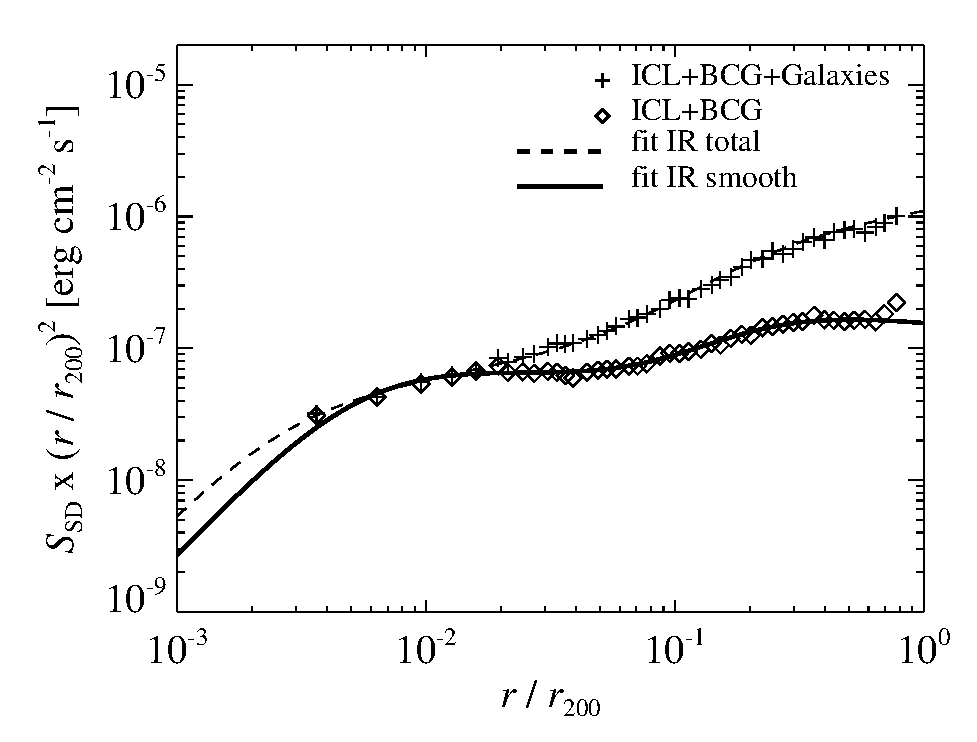
\includegraphics[width=0.99\columnwidth]{figures/SB.photon.eps}
\caption{\it Spatial dependence of light from dust and stars. We show
  2D surface brightness profiles obtained from stacked clusters in the
  Sloan Digital Sky Survey (SDSS) at the redshift $z \sim 0.25$
  \cite{2005MNRAS.358..949Z}. The brightness profiles have been
  weighted with the $\rvir$ normalized area inside radius $r$, and
  trace the radial dependence of the luminosity from stars and
  galaxies. The crosses show the total observed light including the
  diffuse intracluster (ICL), the galaxies, and the brightest cluster
  galaxy (BCG) in the center of the cluster. The diamonds denote the
  observed light from the ICL and the BCG. The solid line show the fit
  to the data of the total light including the ICL, the BCG, and the
  galaxies, while the smooth component is represented by the dashed
  line that is fitted to only the ICL and the BCG.}
 \label{fig3}
\end{figure}

\begin{figure}%[t]
 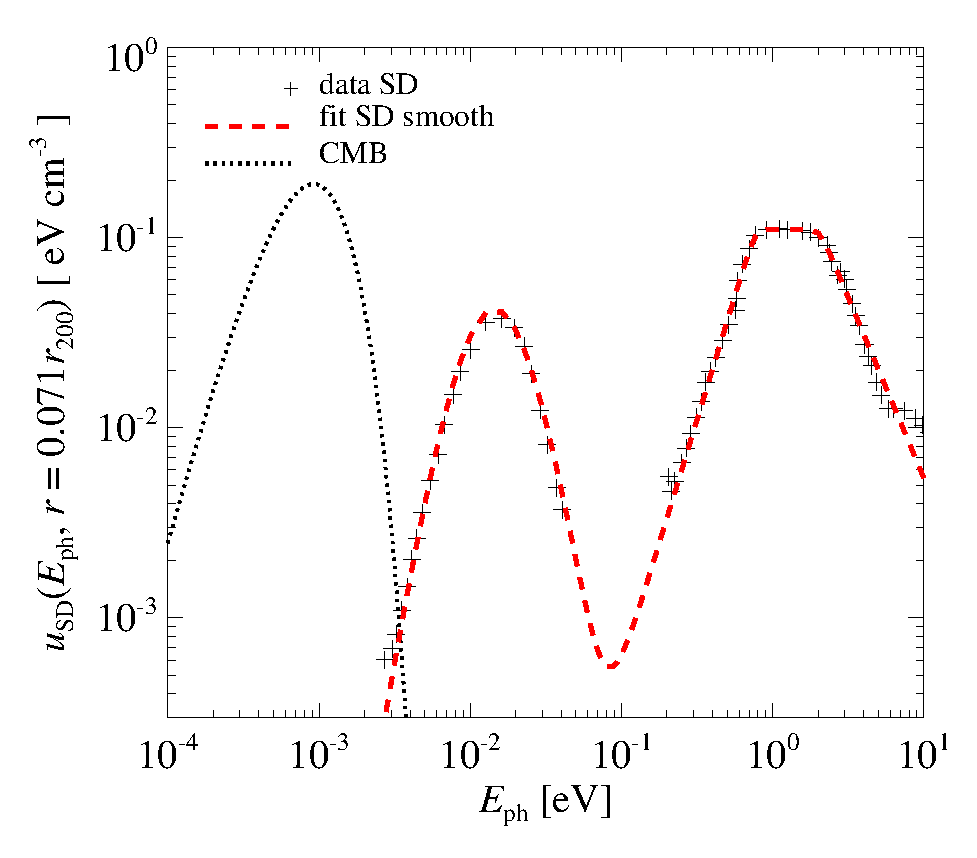
\includegraphics[width=0.99\columnwidth]{figures/fit.porter.v2.eps}
\caption{\it Spectral dependence of radiation fields in a cluster of
  galaxies. The black dotted line in the left peak show the spectrum
  of CMB photons using a black body with a temperature of 2.7 K. The
  crosses in the middle and right peaks represent the measured spectra
  from dust and stars (SD), respectively, and are derived in
  \cite{2006ApJ...648L..29P} for a galaxy. We normalize the individual
  spectra from SD separately using the observed luminosity from SD in
  clusters. The SD luminosity is related to the cluster mass through
  Eqn, where we use have used the mass $\mvir=4.0\,10^{13}\msun$ in this
  figure. Finally we renormalize the SD spectra to the radius
  $r=0.071\rvir$, where the smooth energy density of the SD light (see
  fig~\ref{fig3}) equals the energy density of the CMB. The red dashed
  lines show the fitted SD spectral model.}
 \label{fig4}
\end{figure}

\begin{figure}%[t]
 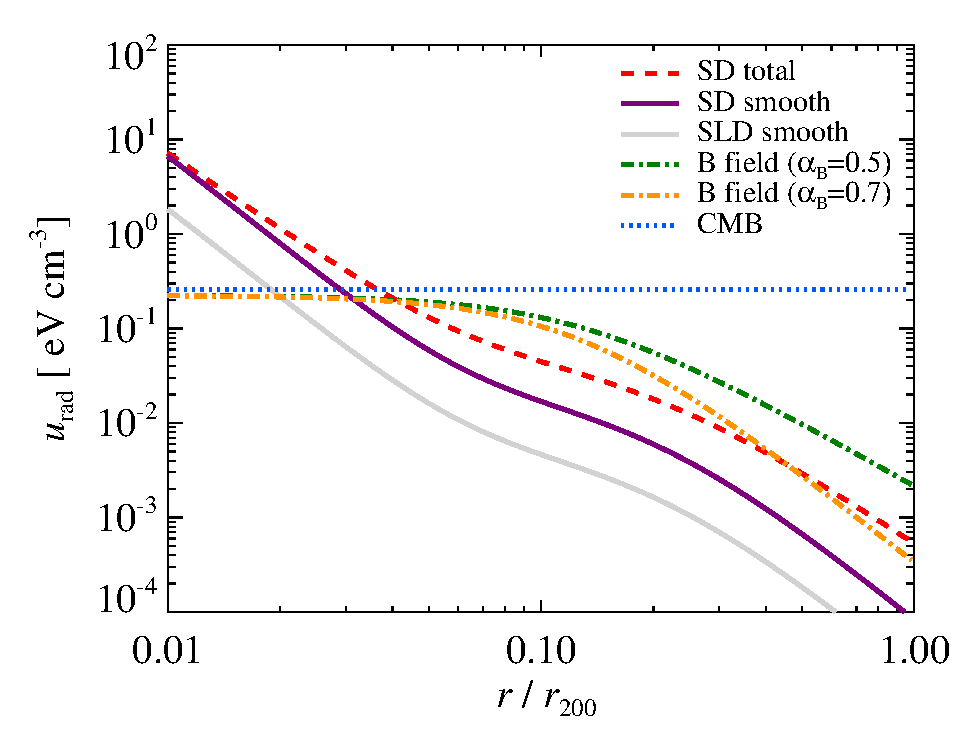
\includegraphics[width=0.99\columnwidth]{figures/ucool.eps}
\caption{\it Spatial dependence of the energy density of radiation
  fields in a cluster of galaxies. The energy density of the CMB, shown
  by the blue dotted line, is isotropic throughout the cluster, hence
  represented by a flat profile with
  $u_\rmn{cmb}=0.26\,\rmn{eV}\,\rmn{cm}^{-3}$. The energy density of
  the light from dust and stars (SD) is denoted by the red dashed line
  and the solid purple line for the total SD light and the smooth SD
  light, respectively. The SD light has been renormalized to a cluster
  with the mass $\mvir=4.0\,10^{13}\msun$. Finally we show the energy density
  two magnetic field models with a central magnetic field of 3~$\mu
  G$. The magnetic field scales with the gas density to the power
  $\alpha_\rmn{B}$; green dash-dotted line ($\alpha_\rmn{B}=0.5$) and
  orange dash-dotted line ($\alpha_\rmn{B}=0.7$). Note that the SD
  radiation is dominating the energy density inside $\sim0.1\,\rvir$.}
 \label{fig5}
\end{figure}


\begin{figure*}
\begin{minipage}{2.0\columnwidth}
 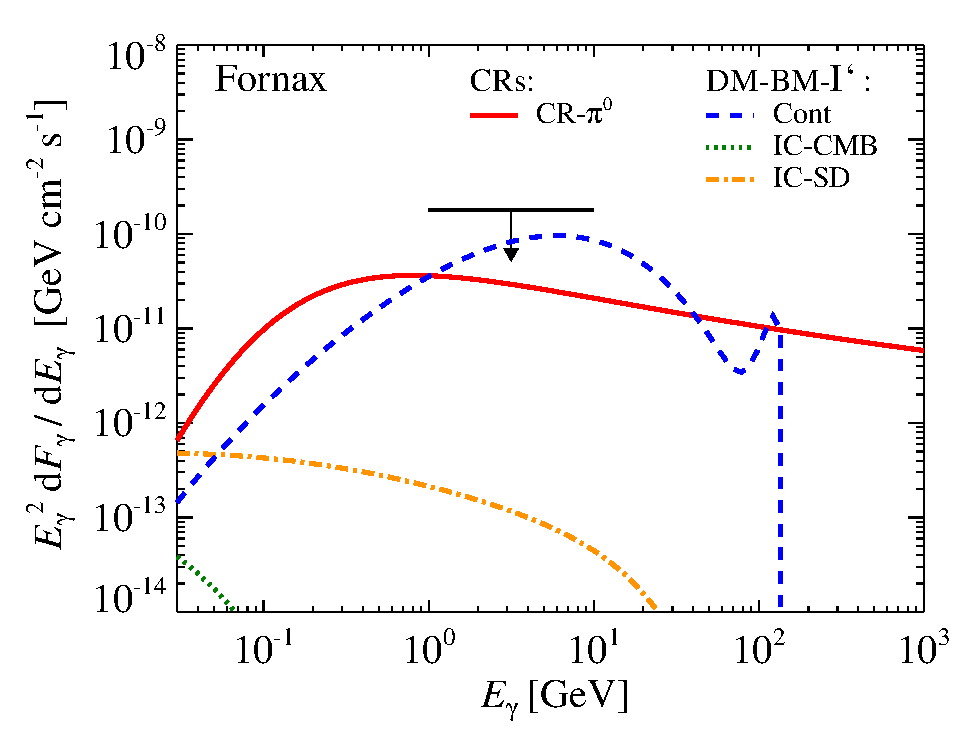
\includegraphics[width=0.49\columnwidth]{figures/flux.BMcompI.v8.0.1deg.1.6T.SubMass.IR2.noMW.woGal.eps}
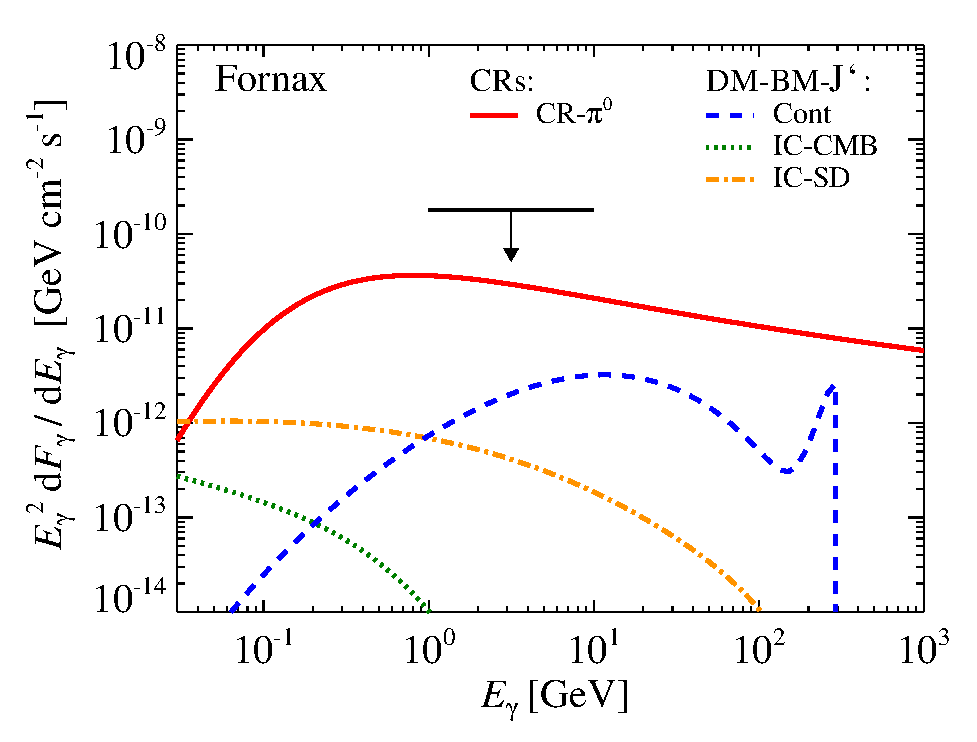
\includegraphics[width=0.49\columnwidth]{figures/flux.BMcompJ.v8.0.1deg.1.6T.SubMass.IR2.noMW.woGal.eps}
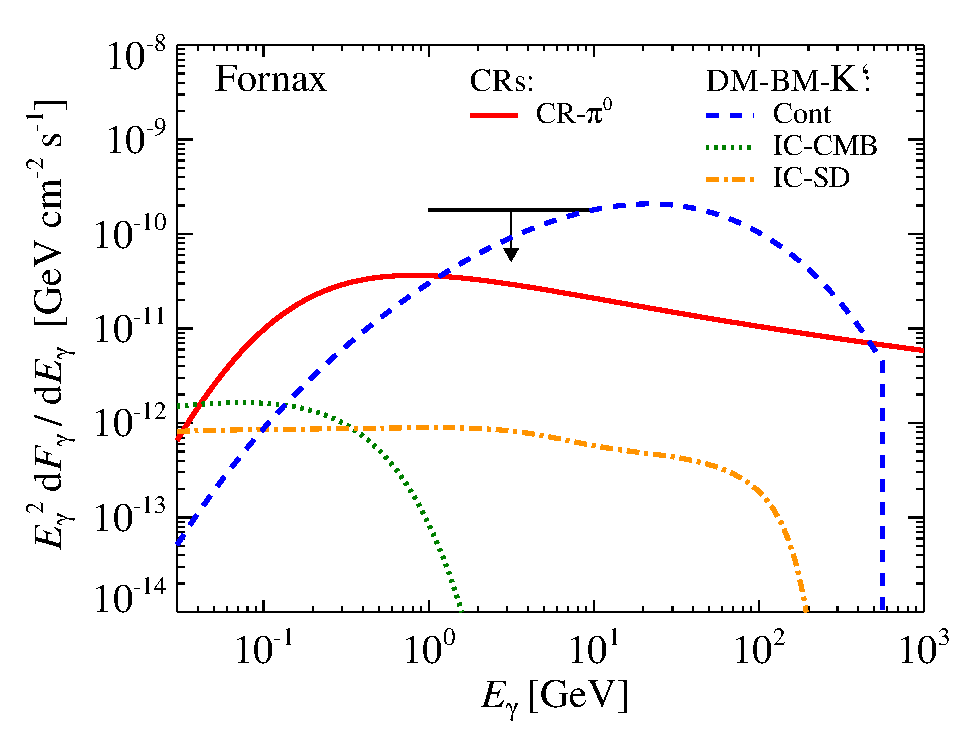
\includegraphics[width=0.49\columnwidth]{figures/flux.BMcompK.v8.0.1deg.1.6T.SubMass.IR2.noMW.woGal.eps}
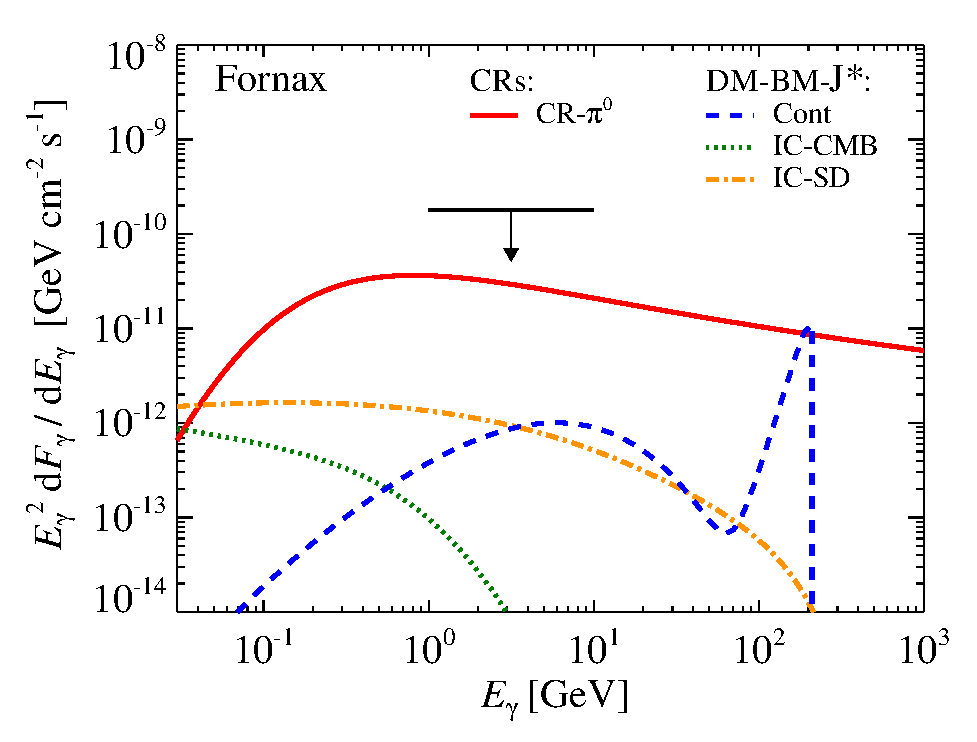
\includegraphics[width=0.49\columnwidth]{figures/flux.BMcompJs.v8.0.1deg.1.6T.SubMass.IR2.noMW.woGal.eps}
\caption{\it Comparing the differential flux from different models: we
  show the continuum emission from DM benchmark (BM) models
  (blue), electrons and positrons from DM BM models that inverse
  Compton upscattered both CMB photons (orange) as well as dust and
  star photons (green), and CR induced gamma-ray emission (red
  solid). The various linestyles are associated with individual DM BM
  models; $\Imm$ (dotted), $\Km$ (dashed), and $\Jm$
  (dash-dotted). The emission is calculated for the Fornax cluster
  using a point spread function of $0.1\deg$ and a boost from
  substructures of ...  We find bright prospects for detecting the
  continuum emission that is dominating the total emission in the GeV
  energy range. Also note that, above 100 MeV the total inverse
  Compton emission is at least a factor 10 smaller than the emission
  expected from both the continuum emission and the emission coming
  from CRs.}
 \label{fig7}
\end{minipage}
\end{figure*}

\begin{figure*}
\begin{minipage}{2.0\columnwidth}
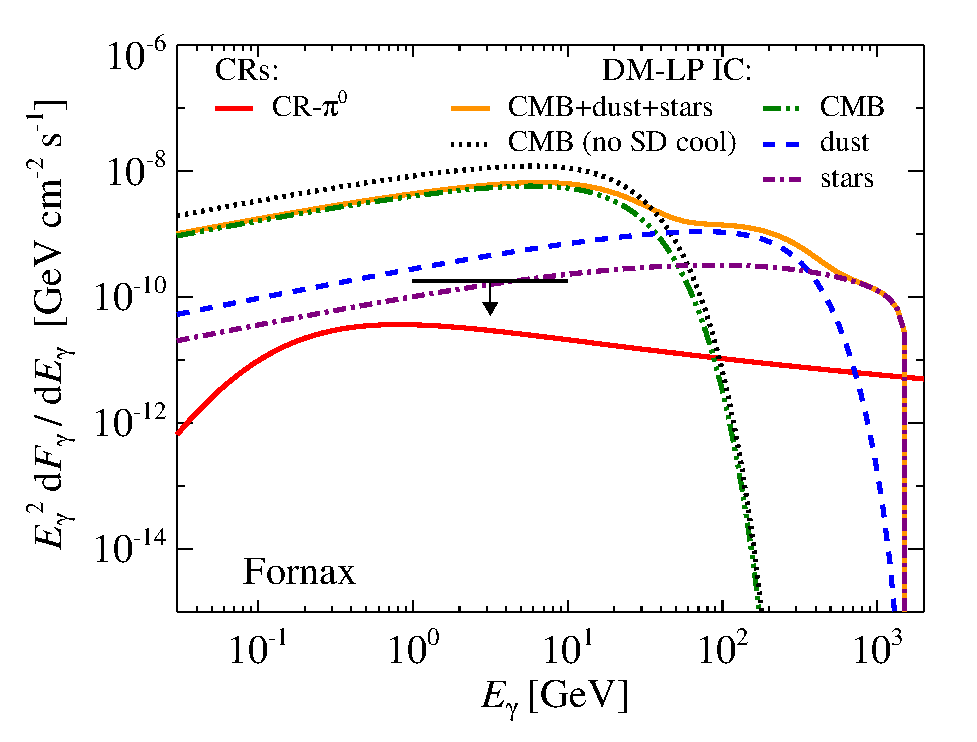
\includegraphics[width=0.49\columnwidth]{figures/flux.IRcomp.v8.0.1deg.1.6T.SubMass.elmu.SF300.noMW.woGal.eps}
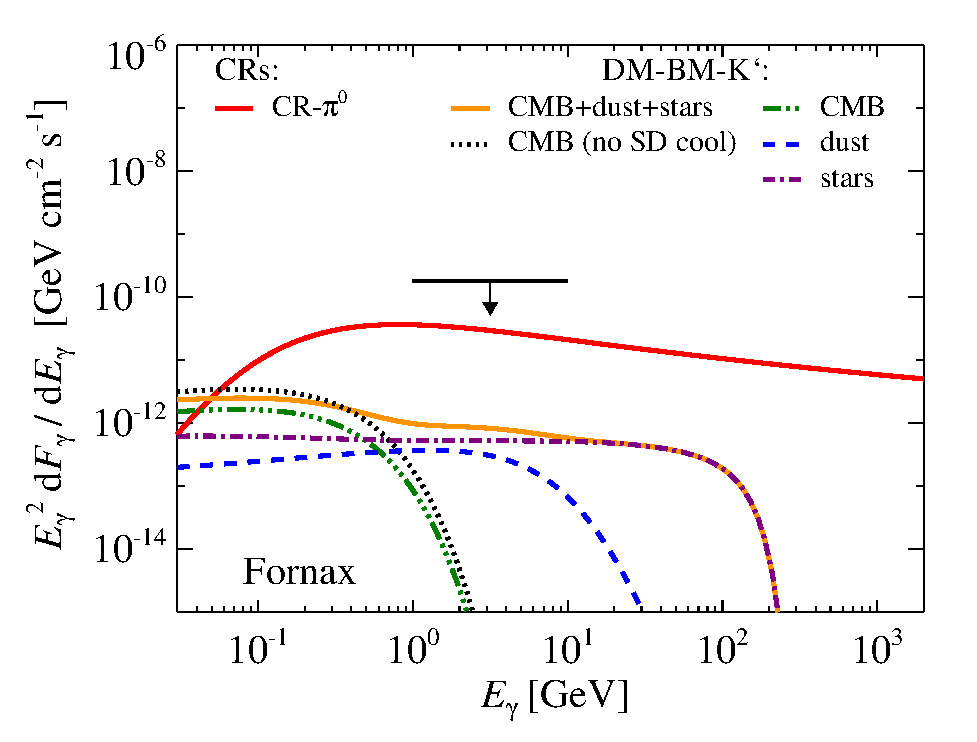
\includegraphics[width=0.49\columnwidth]{figures/flux.IRcomp.BMv8.0.1deg.SubMass.noMW.woGal.eps}
\caption{\it Comparing the differential flux from different inverse
  Compton upscattered radiation fields in the Fornax cluster. We show
  the inverse Compton emissin induced by leptophilic DM in the left
  panel and by the $\Km$ benchmark model in the right panel. The
  contribution from each individual radiation field from top line to
  bottom line; CMB (green dashed-double-dotted), dust (blue dashed),
  stars (purple dashed-dotted). The sum of the three components are
  shown with the orange solid line. The black dotted line represents
  the upscattered CMB photons without any cooling from dust and
  stars. The red solid line show the CR induced gamma-ray flux. The
  black arrow show the differential upper limit from Fermi ADD
  REF. All fluxes are calculated within $\rvir$ with a point spread
  function of $0.1\deg$. The boost from Sommerfeld is ..., and from
  substructures is .}
 \label{fig6}
\end{minipage}
\end{figure*}

\begin{figure}
 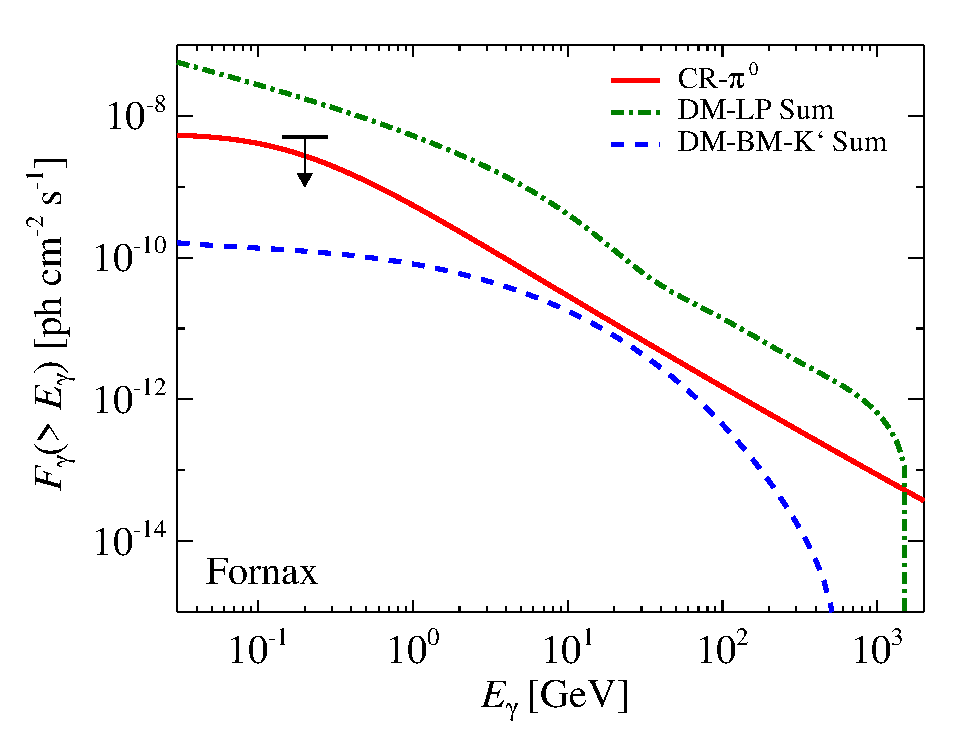
\includegraphics[width=0.99\columnwidth]{figures/flux.int.v8.0.1deg.1.6T.SubMass.SF300.IR2.noMW.woGal.eps}
\caption{\it Comparing the energy integrated flux from different
  models: we show the emission from leptophilic (LP) models with green
  lines, $\Km$ benchmark model (BM) with blue lines, and the CR
  induced emission with a red line. The dotted and dashed lines show
  the inverse Compton (IC) upscattered CMB photons and star and dust
  photons, respectively. The green solid line show the final state
  radiation from the LP model, and the solid blue line show the
  continuum emission from the DM. The black arrow show the integrated
  flux upper limit set by Fermi.  The emission is calculated for the
  Fornax cluster using a point spread function of $0.1\deg$ and a
  boost from substructures of ...  We find that LP models are
  dominating the total flux in the entire energy range, where the IC
  upscattered CMB photons overproduce the upper limit by a factor 3.}
 \label{fig8}
\end{figure}

\begin{figure*}
\begin{minipage}{2.0\columnwidth}
 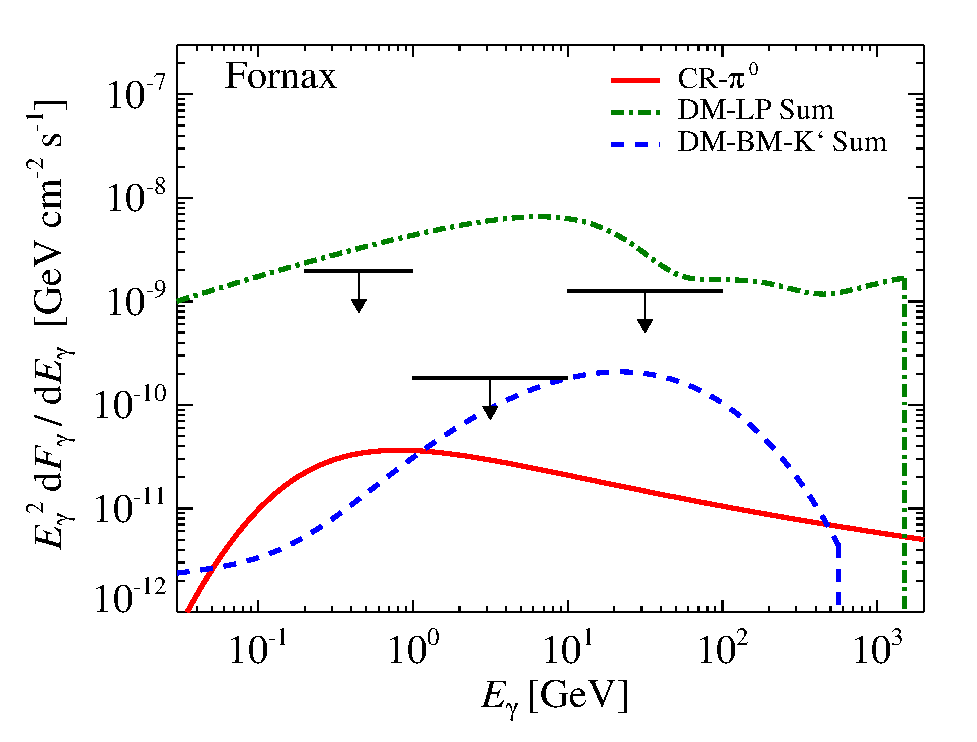
\includegraphics[width=0.49\columnwidth]{figures/flux.cluster.Fornax.v8.0.1deg.1.6T.SubMass.SF300.IR2.noMW.woGal.eps}
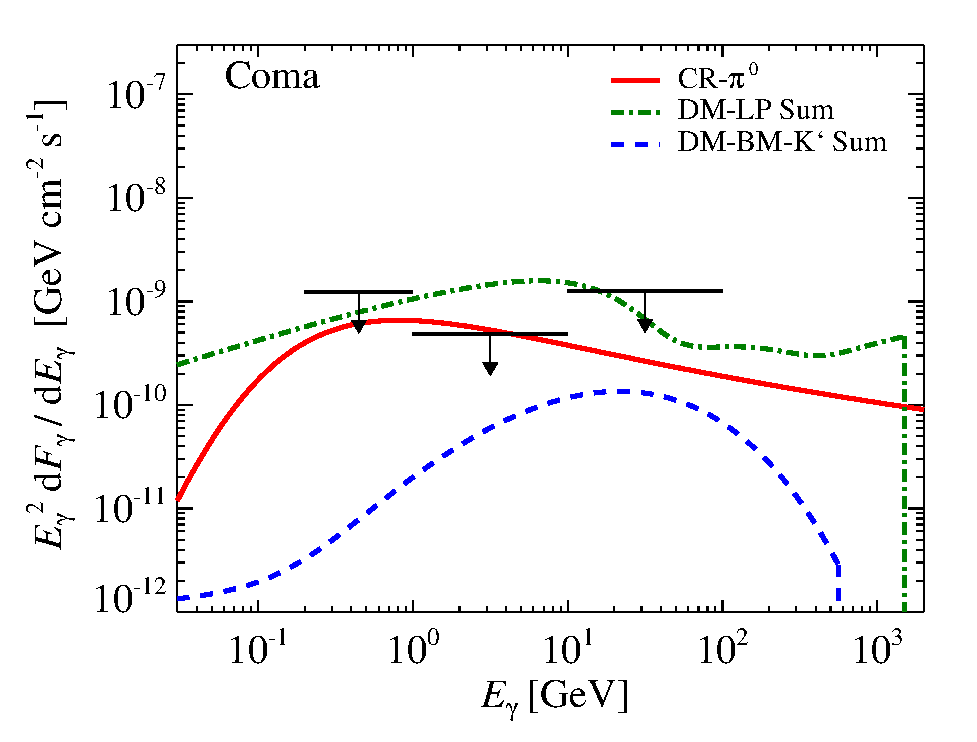
\includegraphics[width=0.49\columnwidth]{figures/flux.cluster.Coma.v8.0.1deg.1.6T.SubMass.SF300.IR2.noMW.woGal.eps}
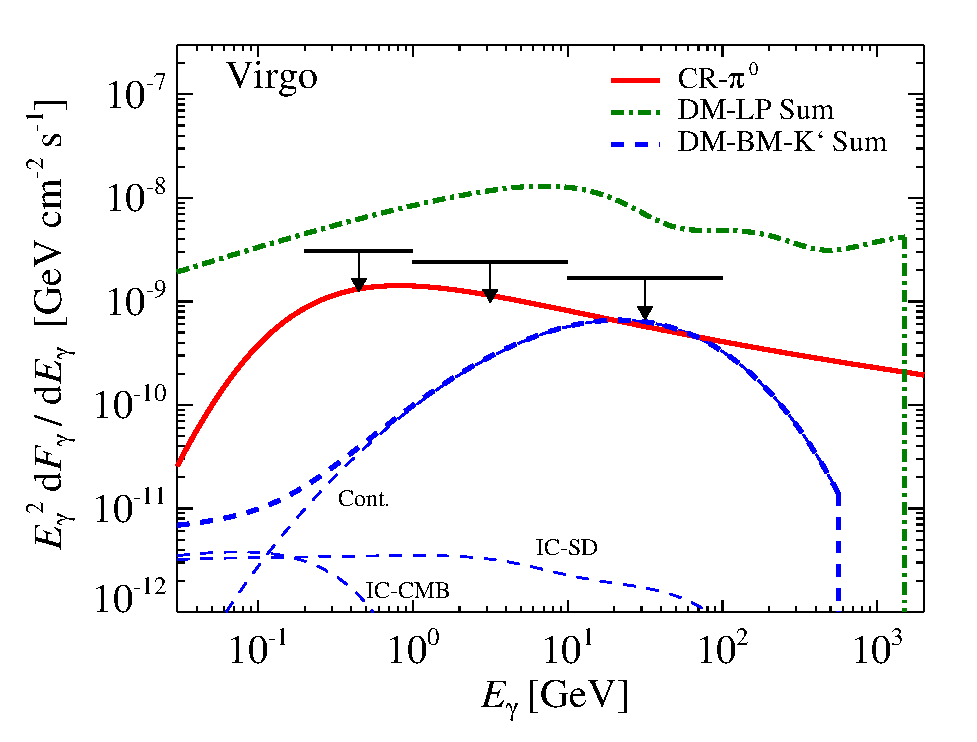
\includegraphics[width=0.49\columnwidth]{figures/flux.cluster.Virgo.v8.0.1deg.1.6T.SubMass.SF300.IR2.noMW.woGal.eps}
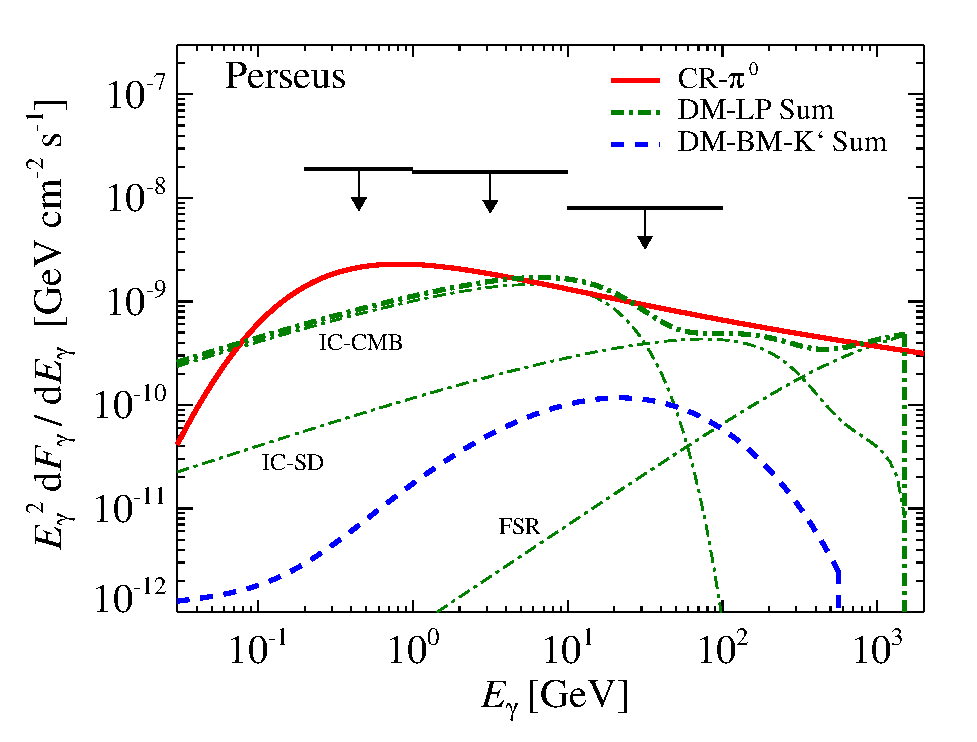
\includegraphics[width=0.49\columnwidth]{figures/flux.cluster.Perseus.v8.0.1deg.1.6T.SubMass.SF300.IR2.noMW.woGal.eps}

\caption{\it Comparing the emission from different clusters. The
  emission from the clusters is calculated using a point spread
  function of $0.1\deg$ and includes the boost from substructures. We
  show the differential flux from four clusters; Fornax (upper left),
  Coma (upper right), Virgo (lower left), and Perseus (lower
  right). The different linestyles show; CR induced emission (solid),
  leptophilic models (LP) include both final state radiation and IC
  upscattered CMB, dust and star light (dotted), and benchmark $\Km$
  models (BM) include continuum emission, and IC upscattered CMB, dust
  and star light (dashed). The arrows have colors matching each
  cluster and show the differential upper limits set by Fermi in the
  energy ranges $0.2-1$~GeV, $1-10$~GeV, and $10-100$~GeV from left to
  right. For visualization we offset the arrows by increasing the mean
  energy by 30 percent in the opposite order as they appear in the
  figure, i.e. starting with Perseus. All fluxes are calculated within
  $\rvir$. We find that the lower GeV energy regime is most
  constraining, and induce upper limits on boost factors.}
 \label{fig9}
\end{minipage}
\end{figure*}

\begin{figure}
 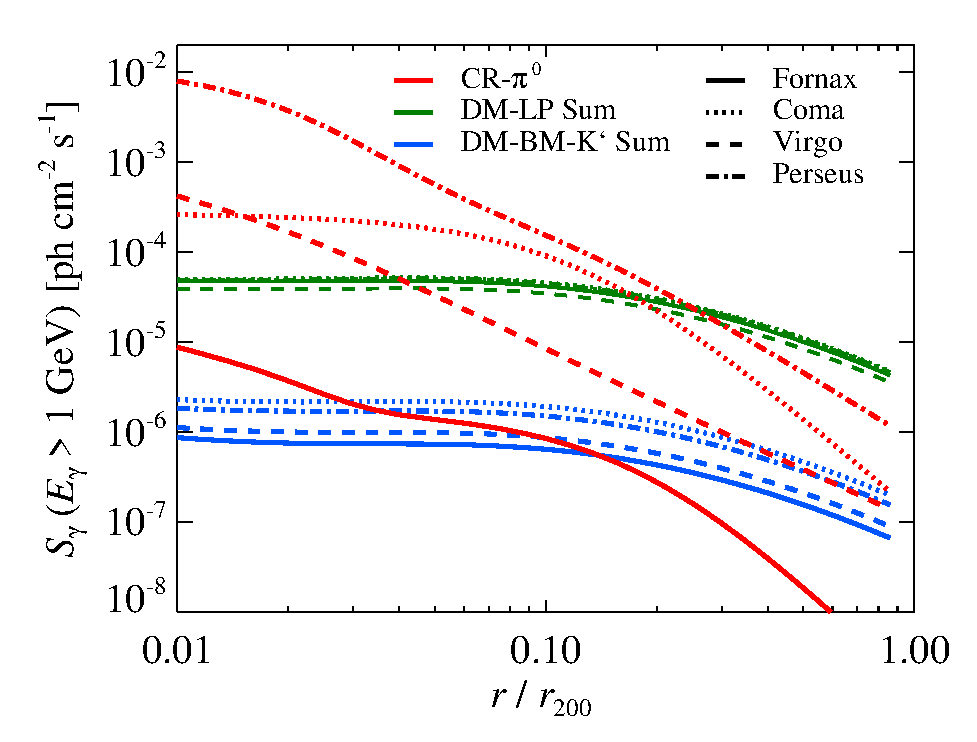
\includegraphics[width=0.99\columnwidth]{figures/SB.v8.1GeV.SF300.SubMass.elmu.eps}
\caption{\it Comparing the surface brightness from different
  clusters. We show the surface brightness above the energy 1~GeV. The
  boost from substructures is included and we usie a point spread
  function of $0.1\deg$.}
 \label{fig20}
\end{figure}

\begin{figure}%[t]
 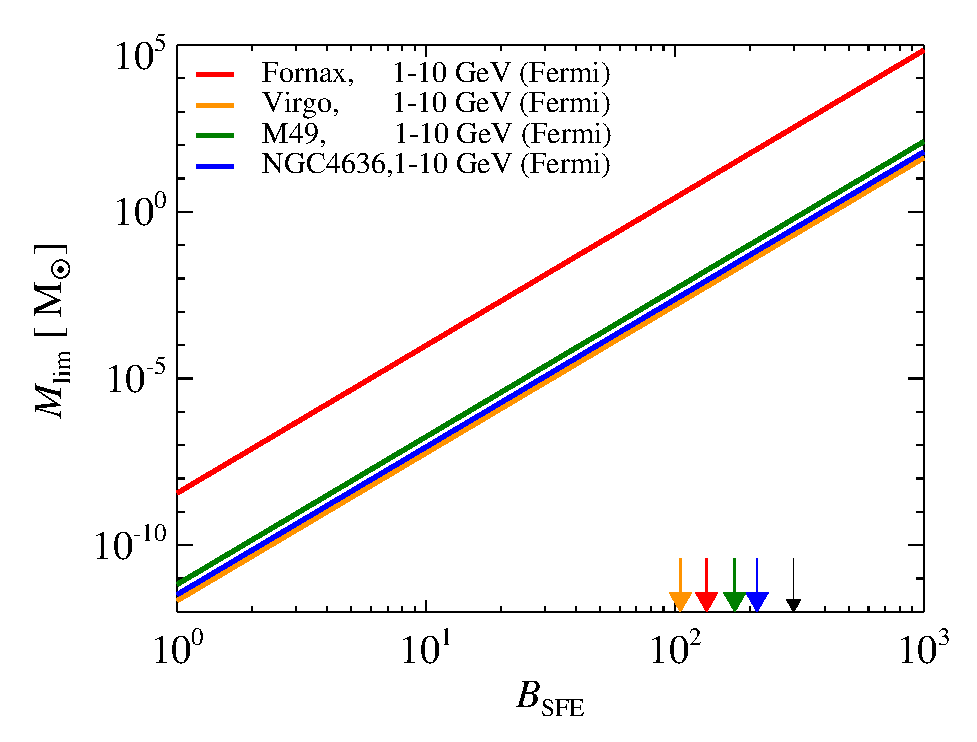
\includegraphics[width=0.99\columnwidth]{figures/LP.const.diff.v8.0.1deg.1.6T.SubMass.SF300.IR2.noMW.woGal.eps}
\caption{\it Constraining leptophilic boost factors using flux upper
  limits. The emission is derived within $\rvir$ using a point spread
  function of $0.1\deg$. In order not to overproduce the Fermi
  differential flux upper limits in the energy interval $1-10$~GeV the
  boost from substructures and Sommerfeld enhancement (SFE) is
  constrained for four clusters; Fornax (red), Virgo (orange), M49
  (green), and NGC4636 (Blue). The arrows have colors matching each
  cluster and indicate the SFE in each cluster. The SFE has been
  rescaled from 300 that is required to explain the electron and
  positron excess observed in the Milky Way (MW) with leptophilic dark
  matter (refer to equation). If the DM interpretation is correct, we
  can constrain the smallest size of halos to be larger than
  $10\,\msun$. However, if the smallest size of DM halos is
  $10^{-6}\,\msun$, we can constrain the SFE to about 4 in Fornax,
  corresponding to a maximum SFE in the MW of about 10.}
 \label{fig10}
\end{figure}

\begin{figure}%[t]
 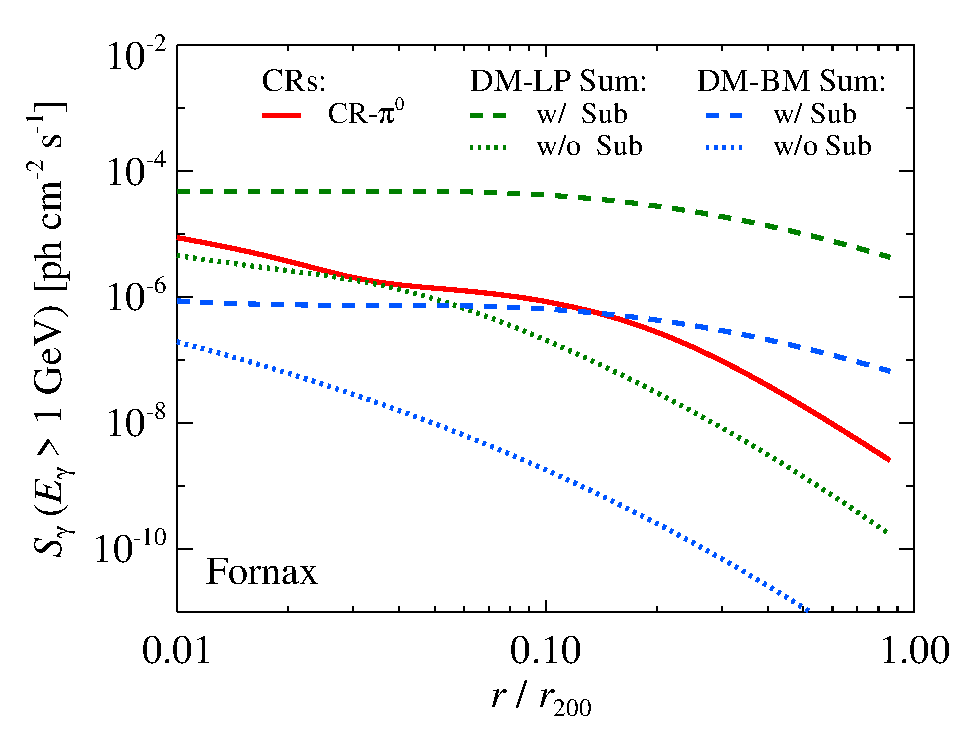
\includegraphics[width=0.99\columnwidth]{figures/SB.resolved.v8.1GeV.SF300.noSuB.vs.SubMass.elmu.eps}
\caption{\it The impact of substructures on surface brightness. We
  show the surface brightness at 1~GeV for the Fornax cluster using a
  very small point spread function of $10^{-5}\deg$ that reveals the
  details of the spatial profiles. The emission induced by CRs is
  denoted by the red solid line, the leptophilic models by green
  lines, and the DM $\Km$ benchmark model by blue lines. The dashed
  and dotted lines include and exclude substructures,
  respectively. Notice the nearly flat profiles when substructures are
  included, and the relative large boost at a percent of $\rvir$.}
 \label{fig11}
\end{figure}

\begin{figure*}
\begin{minipage}{2.0\columnwidth}
  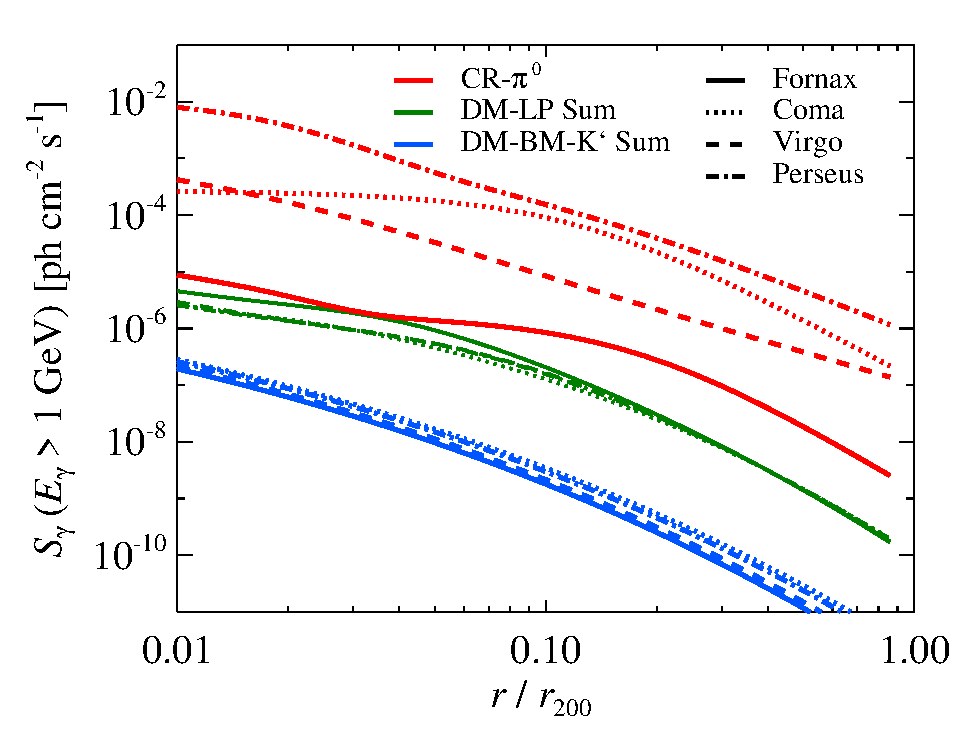
\includegraphics[width=0.49\columnwidth]{figures/SB.v8.1GeV.SF300.noSuB.elmu.eps}
  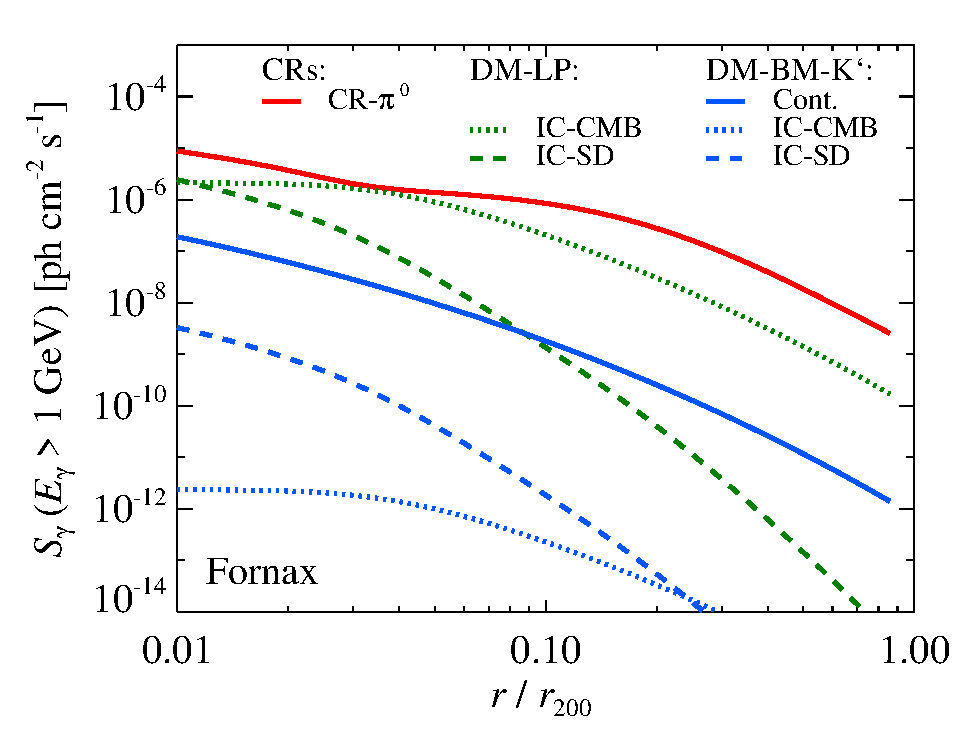
\includegraphics[width=0.49\columnwidth]{figures/SB.fornax.v8.1GeV.SF300.noSuB.elmu.eps}
\caption{\it The surface brightness without substructures. We show the
  CR induced emission (red), leptophilic emission (green), and
  emission from the $\Km$ benchmark model (blue). The surface
  brightness above 1~GeV is derived using a very small point spread
  function ($\theta_\rmn{psf}=10^{-5}\deg$). LEFT PANEL: compare the
  surface brightness for different clusters; Fornax (solid), Coma
  (dotted), Virgo (dashed), and Perseus (dash-dotted).  RIGHT PANEL:
  compare different emission components in Fornax; dotted lines show
  the inverse Compton (IC) upscattered CMB photons, dashed lines show
  the IC upscattered photons from dust and stars, and blue solid line
  show the continuum emission from the $\Km$ benchmark
  model. \del{Since cooling is dominated by IR and UV processes in the
    center, the spatial dependence of the equilibrium electron spectra
    cancels the spatial dependence on the upscattered IR photon,
    resulting in a smooth halo dependence (density square) in the
    center. The spatial profile for the upscattered CMB photons is
    flatter in the center since the strong spatial dependence inferred
    from cooling counteracts the smooth halo contribution. Cluster
    outskirts dominated by the emission from DM, although large
    uncertainty in the gas density profile.}}
 \label{fig12}
\end{minipage}
\end{figure*}

\begin{figure*}
\begin{minipage}{2.0\columnwidth}
  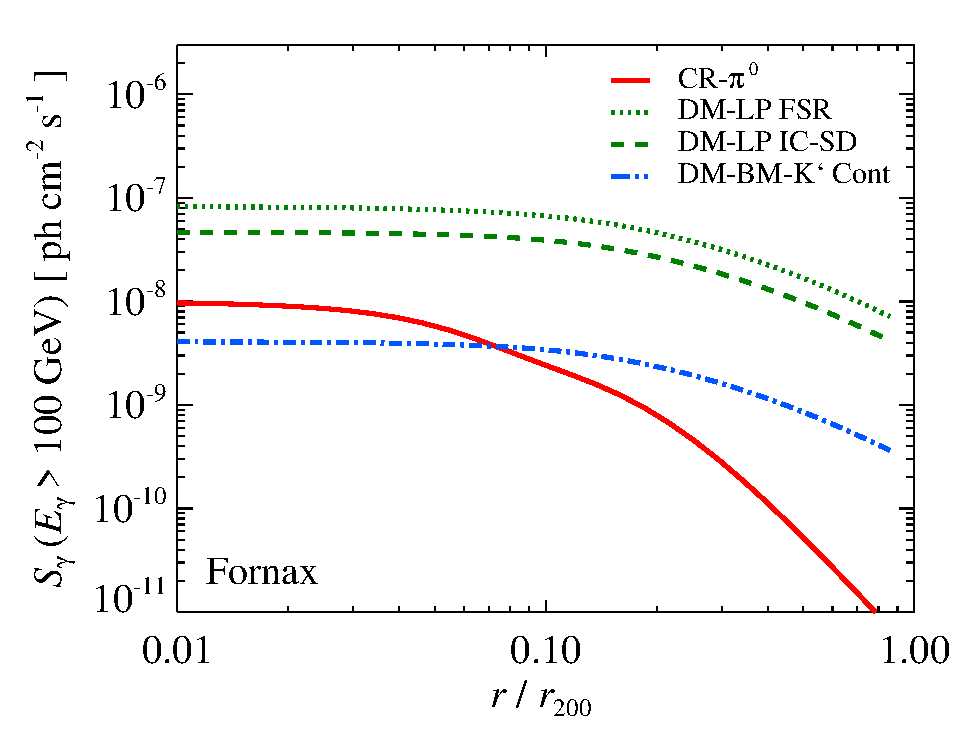
\includegraphics[width=0.49\columnwidth]{figures/SB.Fornax.v8.SF300.SubMass.elmu.eps}
  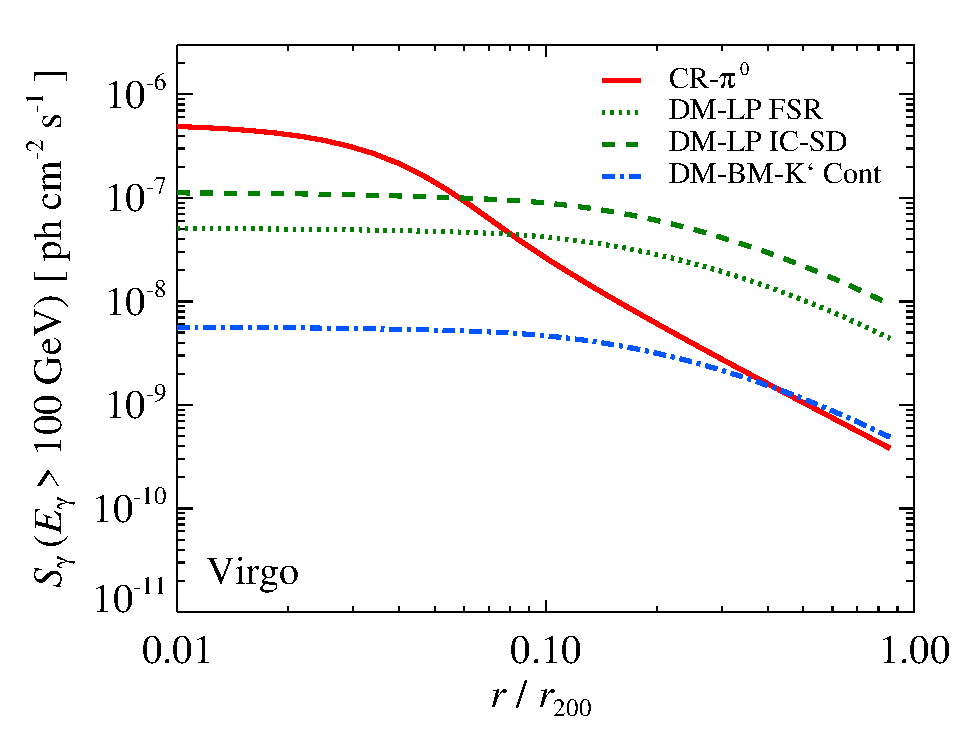
\includegraphics[width=0.49\columnwidth]{figures/SB.Virgo.v8.SF300.SubMass.elmu.eps}
\caption{\it Surface brightness predicted for Cherenkov telescopes. We
  show the emission above $\eg=100$~GeV, include the boost from
  substructures and use a point spread function of $0.1\deg$. Left
  panel show the Fornax cluster and right panel the Virgo cluster. The
  emission is derived for the following components; CRs (red solid),
  continuum emission from the DM $\Km$ benchmark model (blue
  dash-dotted), as well as final state radiation (green dashed) and
  inverse Compton upscattered dust and star light (green dotted) from
  leptophilic DM. \del{GeV energies give rise to small BM model fluxes
    but high LP fluxes, other words BM models good for Cerenkov
    telescopes and LP good for Fermi (although the flat LP spectra
    give rise to high fluxes at high energies as well).}}
 \label{fig13}
\end{minipage}
\end{figure*}

\begin{figure*}
\begin{minipage}{2.0\columnwidth}
  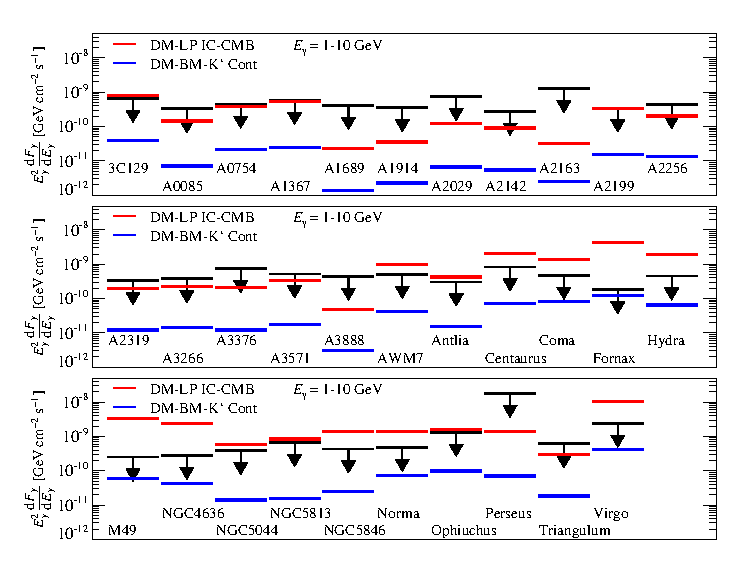
\includegraphics[width=0.99\columnwidth]{figures/Fermi.comp.DM.eps}
  \caption{\it Fermi flux upper limits contrasted to the predicted DM
    gamma-ray flux. We show the mean differential flux in the energy
    range $E_\gamma=1-10$~GeV for 32 clusters. The Fermi upper limits
    are shown with black arrows. The predicted fluxes are derived from
    both a leptophilic DM model that result in inverse Compton
    upscattered CMB photons (red), and the continuum emission from the
    DM $\Km$ benchmark model (blue). The leptophilic fluxes are ruled
    out by 14 of the clusters, with the strongest constraints set by
    Fornax and M49. We can not constrain the benchmark models,
    although our predictions are approaching the upper limits.}
 \label{fig14}
\end{minipage}
\end{figure*}

\begin{figure*}
\begin{minipage}{2.0\columnwidth}
  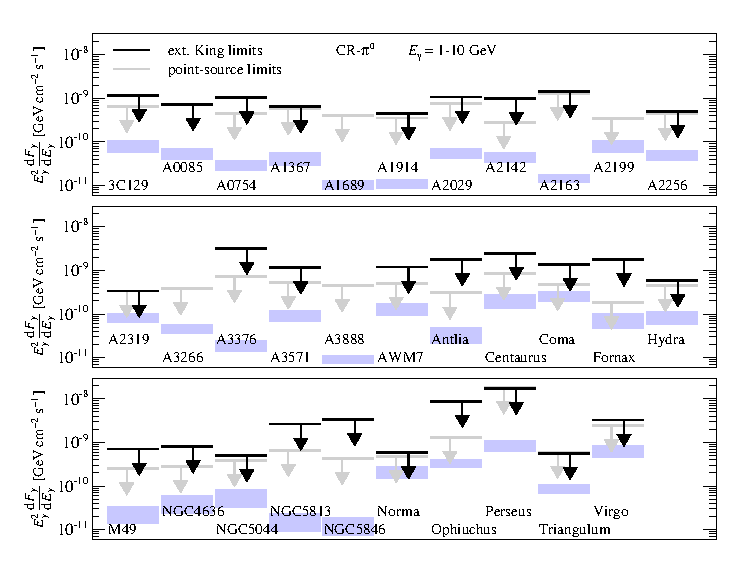
\includegraphics[width=0.99\columnwidth]{figures/Fermi.comp.CR.diff.eps}
  \caption{\it Fermi flux upper limits contrasted to the predictions
    by the semi-analytic Pinzke and Pfrommer model for CR induced
    gamma-ray emission. We show the mean differential flux in the
    energy range $E_\gamma=1-10$~GeV for 32 clusters. The Fermi upper
    limits are shown with black arrows. The blue boxes show the
    gamma-ray emission from CR induced $\pi^0$\:s decaying, where the
    upper bound shows the estimates for an optemistic model and the
    lower bound a more conservative model excluding point sources (the
    realistic case is more likely in between, see
    \cite{2010MNRAS.409..449P} for details). Note that there is
    currently no tension between our predictions and upper limits from
    Fermi, although Virgo, Norma, and Coma are close and will in the
    coming years enforce constraints on the hadronic models.}
 \label{fig15}
\end{minipage}
\end{figure*}


%------------------------------------------------------------------


\smallskip
We wish to thank...

%%%%%%%%%%%%%%%%%%%%%%%%%%%%%%%%%%%%%%%%%%%%%%%%%%%%%%%%%%%%%%%
\vspace{-0.7cm}
\bibliography{bibtex/paper}
%\bibliography{apssamp}
%\bibliographystyle{apsrev4-1}

\clearpage
\appendix

\begin{figure*}
\begin{minipage}{2.0\columnwidth}
 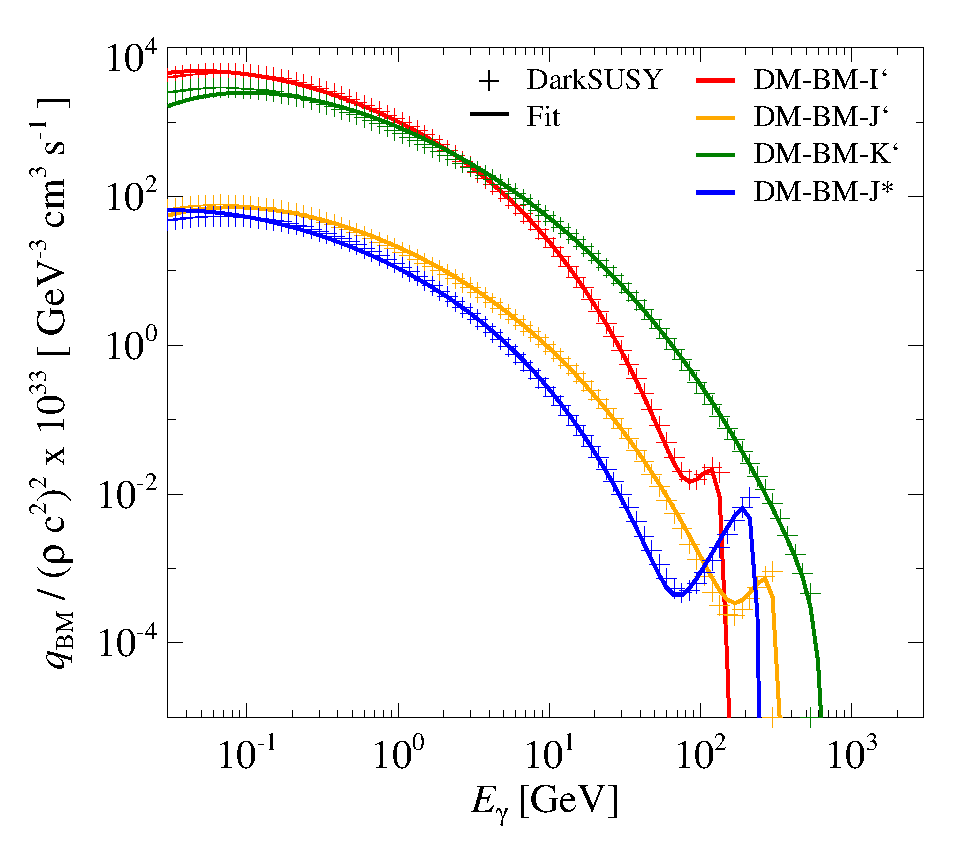
\includegraphics[width=0.49\columnwidth]{figures/fit.ds.flux.eps}
 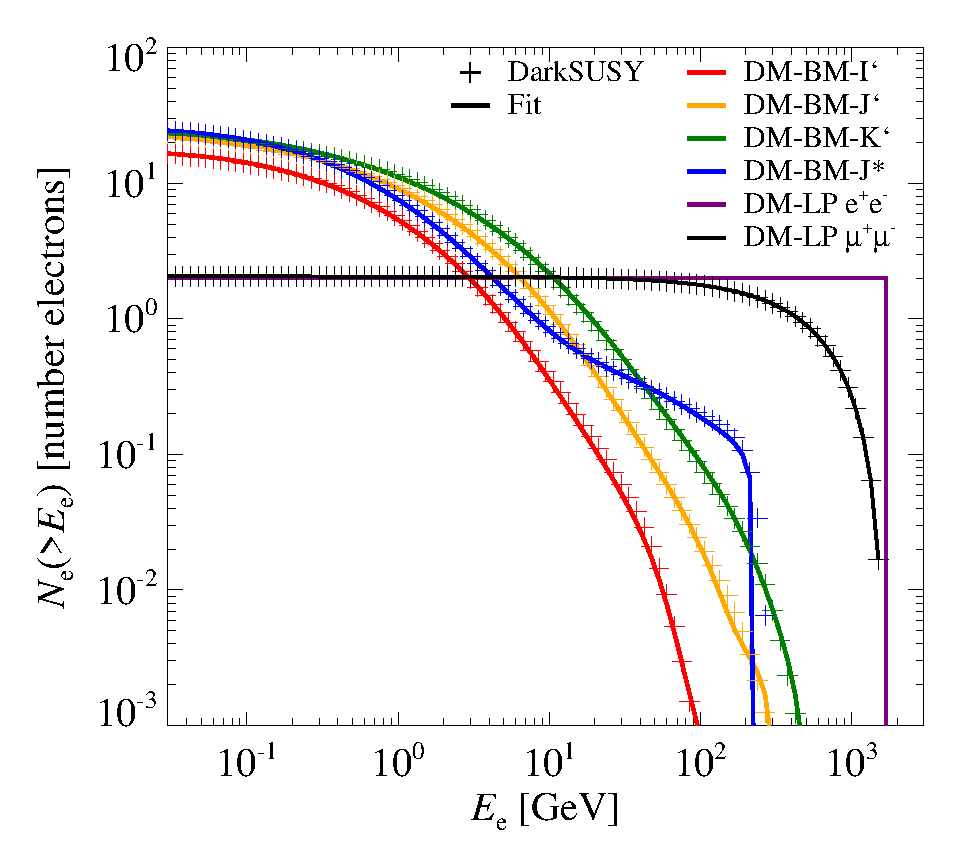
\includegraphics[width=0.49\columnwidth]{figures/fit.epflux.int.eps}
\caption{\it The underlying source functions for different DM
  models. Crosses show the simulated data from DarkSUSY and the solid
  lines show the fit to the data using Eqn.... LEFT PANEL: normalized
  differential continuum spectra for four different DM benchmark (BM)
  models; $\Imm$ model (red), $\Jmm$ (orange), $\Km$ (green), and
  $\Jm$ (blue). RIGHT PANEL: number of electron and positron per DM
  annihilation above the electron energy $E_\e$ for different dark
  matter models; $\Imm$ BM model (red), $\Jmm$ BM model (orange),
  $\Km$ BM model (green), and $\Jm$ BM model (blue), leptophilic (LP)
  DM annihilating into electrons and positrons (purple), and LP DM
  annihilating into muons (black).}
 \label{fig17}
\end{minipage}
\end{figure*}

\begin{figure}%[t]
 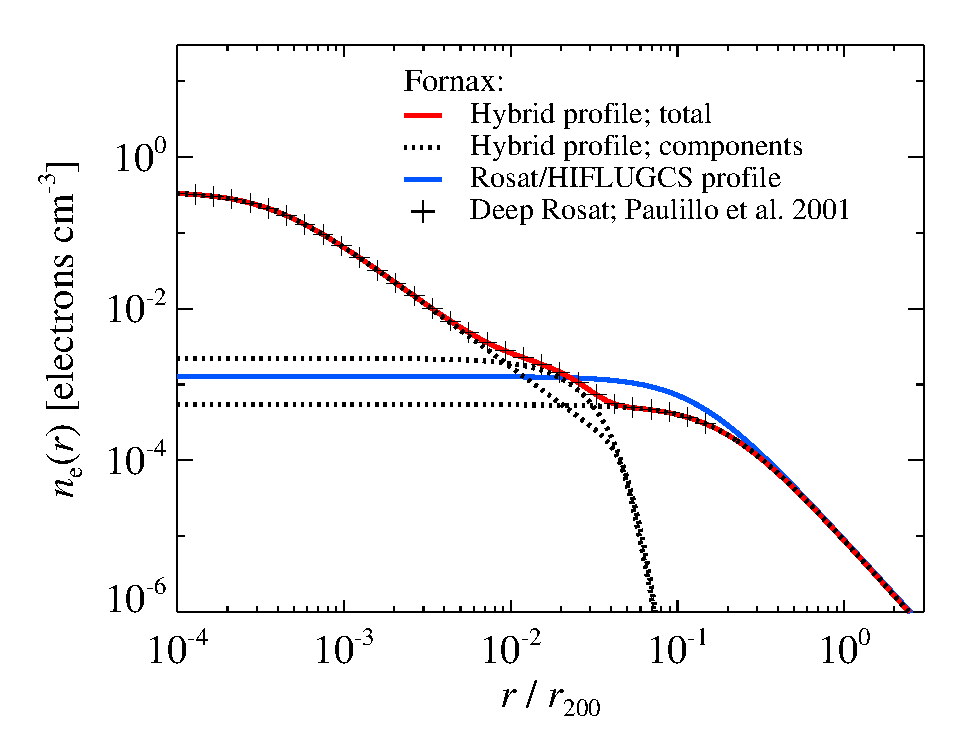
\includegraphics[width=0.99\columnwidth]{figures/dens.fornax.eps}
\caption{\it Comparing different electron number density profiles for
  the Fornax cluster. Black crosses show the density profile inferred
  from deprojected Chandra and Rosat X-ray surface brightness
  observations CITE. The total hybrid profile shown by the red solid
  line represent the best fit to the data, where the fitted individual
  density components are shown by the black dotted lines. The blue
  solid line show the single beta density profile inferred from the
  HIFLUGCS catalogue. Due to insufficient sensitivity to the outer part
  in the plotted data, we infer the outer slope found in the HIFLUGCS
  catalogue.}
 \label{fig18}
\end{figure}


\begin{figure*}%[t]
\begin{minipage}{2.0\columnwidth}
 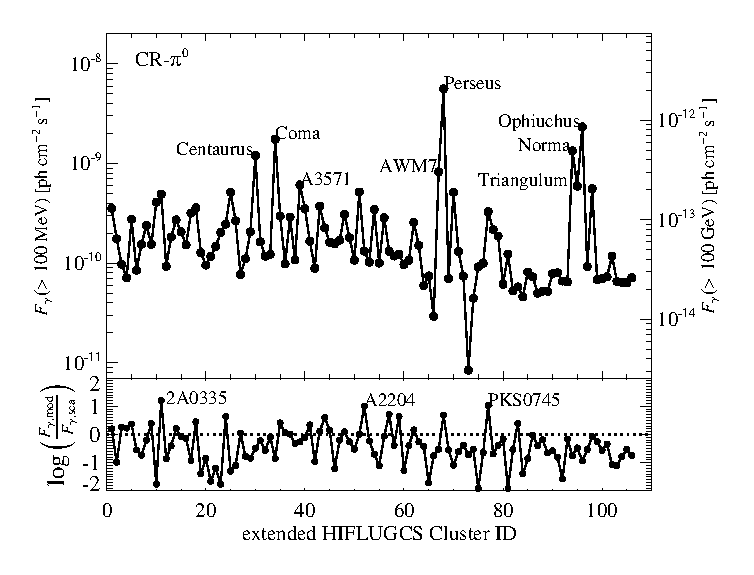
\includegraphics[width=0.99\columnwidth]{figures/Flux.comp.CR.eps}
\caption{\it Comparing the flux from clusters in the extended HIFLUGCS
  catalogue. We show the energy integrated gamma-ray flux induced by
  CRs for the 106 clusters included in the extended HIFLUGCS
  catalogue. The fluxes are calculated within $\rvir$, and are derived
  using a single beta profile for each cluster's gas density profile
  (see text for details). The upper panel show the energy integrated
  flux above 100~MeV (left side) and above 100~GeV (right side), both
  as a function of HIFLUGCS cluster ID. The name of the eight
  brightest clusters are written out. The lower panel show the
  relative difference between the gamma-ray flux predicted by
  mass-luminosity scaling relations compared to the flux computed
  using the semi-analytically model CITE The name of the
  clusters with the largest offset are printed out, which correlate
  with cool core clusters.}
 \label{fig19}
\end{minipage}
\end{figure*}

\begin{figure*}%[t]
\begin{minipage}{2.0\columnwidth}
 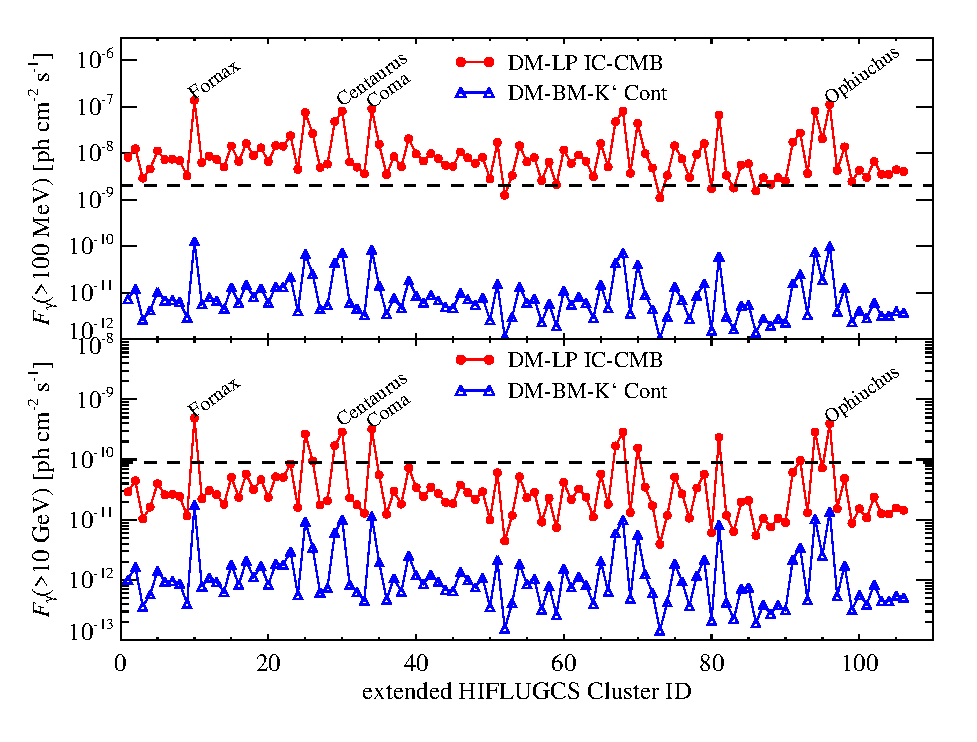
\includegraphics[width=0.99\columnwidth]{figures/Flux.comp.DM.eps}
\caption{\it Comparing the flux from clusters in the extended HIFLUGCS
  catalogue. We show the energy integrated gamma-ray fluxes derived
  from both leptophilic DM that result in inverse Compton upscattered
  CMB photons (red), and the continuum emission from the DM $\Km$
  benchmark model (blue). The fluxes are calculated within $\rvir$
  for each of the 106 clusters included in the extended HIFLUGCS
  catalogue, and are derived using a single beta profile for each
  cluster's gas density profile (see text for details). The upper
  panel show the energy integrated flux above 100~MeV and the lower
  panel above 10~GeV, both as a function of HIFLUGCS cluster ID. The
  name of the four brightest clusters are written out, where Fornax
  and M49 are the brightest targets.}
 \label{fig21}
\end{minipage}
\end{figure*}

\end{document}
